\documentclass[12pt]{article}
\usepackage[latin1]{inputenc}
\usepackage{amsmath}
\usepackage{mathtools}
\DeclarePairedDelimiter\Floor\lfloor\rfloor
\DeclarePairedDelimiter\Ceil\lceil\rceil
\usepackage{amsfonts}
\usepackage{amssymb}
\usepackage{graphicx}
\usepackage{natbib}
\usepackage{rotating}
\bibliographystyle{apsr}
\usepackage[hidelinks]{hyperref}
\usepackage[titletoc,title]{appendix}

\usepackage[left=1.0in, right=1.0in, top=1.0in, bottom=1.0in]{geometry}

\author{Jude C. Hays\footnote{Department of Political Science, University of Pittsburgh}, Robert J. Franzese, Jr.\footnote{Department of Political Science, University of Michigan}, Joseph T. Ornstein\footnote{Brown School, Washington University in St. Louis}}
\title{Estimating the Interest-Premium Cost of Left Government by Regression Discontinuity Analysis of Close Elections}


\usepackage{setspace}
\setlength{\parskip}{1.0ex}

\begin{document}

\singlespacing
\maketitle
\doublespacing

\begin{abstract} 
\noindent This paper employs a regression discontinuity design (RDD) to ascertain the effects of left government on the interest-rate premium that markets build into government bond prices. One advantage of this approach is that RDD does not require, as have previously employed strategies, strong assumptions about how market actors form political expectations, about the quality and dissemination of political information, or about functional forms or explanatory-variable selection. Our findings suggest no or very small and insignificant partisan-government effects except under specific circumstances (low fragmentation, high polarization), in certain eras (around the 1950s-1970s), and for a short-term (about one year), under which conditions there is a statistically discernible and substantively notable government-bond yield increase after left parties enter government following close elections.

\end{abstract}

\pagebreak

\section{Introduction}

% Paragraph 1: Introduce the central question -- how do markets react to partisan composition of government?
How do financial markets react to the partisan composition of government? What cost, if any, do citizens pay in higher government bond interest rates for electing left-leaning and social democratic parties? 

% Paragraph 2: Some theories imply a large cost of social democracy
Because social democratic (left) parties tend to support policies that involve the redistribution of wealth, many scholars expect that financial markets will react strongly when such parties are elected to government. The \textit{locus classicus} on the topic is \citet{Lindblom1977} \textit{Politics and Markets}, which emphasizes the ``privileged position of capital'', i.e., capital's ability to withhold investment as a credible threat against governments thinking to act against investors' interests. Proponents of rational partisan theory argue that financial markets impose a high price on citizens who choose center-left representatives \citep{Alesina1997, Herron2000}. 

% Paragraph 3: Other theories imply small or zero cost of social democracy.
Others theories, however, predict a small or zero financial market response to the partisanship of government. Scholars from the varieties of capitalism literature contend that traders only worry about macroeconomic performance and not policy or partisanship \textit{per se} \citep{Clark2003, Mosley2000, Garrett1998}. Since, according to this camp, there is no systematic relationship between partisanship and inflation, the cost of social democracy may be quite low or even negative. Still others maintain that the globalization of financial markets has placed a ``Golden Straightjacket'' on governments, shrinking the policy space between the right and left \citep{Rodrik2000}, or that democratic competition induces a Hotelling-Downsian convergence in the macroeconomic policies of left and right governments \citep{Clark2003}. In either case, financial markets will be indifferent to the partisan composition of government.

% Paragraph 4: Limitations of existing approaches -- OVB and reverse causality
Previous attempts to resolve this question empirically have faced three important limitations. First, omitted variable bias: many potentially observable variables can influence both bond-market performance and the electoral success of parties. For example, oil-price shocks might affect both interest rates and the effectiveness of economic policies in a party's policy toolkit, and thereby its probability of winning elections. Second, reverse causality: bond prices affect right- and left-party core constituencies differently and therefore affect the probability of observing left or right governments. For example, a hypothetical exogenous bond-price appreciation (interest-rate decrease) is macroeconomically stimulatory, and such a stimulus may alter the relative appeal of leftist or rightist platforms and so the probability of a left party election victory. 

% Paragraph 5: Limitations of existing approaches -- structural approaches must explicitly model the expectation formation of traders
A third challenge arises because financial markets are composed of forward-looking political-economic actors. Even in the presence of large treatment effects, na\"ive pre-post comparisons might fail to find partisan-government effects if shifts in government partisanship are long anticipated by traders. Structural approaches to estimation must rest on implausibly restrictive assumptions about the way traders form political expectations \citep{Alesina1997}, posit specific assumptions about the quality and dissemination of political information \citep{Herron2000}, or make debatable specification decisions related to functional forms and variable selection (e.g., \citet{Garrett1998}, \citet{Franzese2002}, \citet{Clark2003}, \citet{Mosley2003}, \citet{Bernhard2006}, to list just a few in this style). As a result, these approaches reach more equivocal and contestable conclusions about ``the price of social democracy''. 



% Paragraph 6: RD overcomes these challenges; introduce our research design
The regression discontinuity design (RDD) offers a method to overcome these challenges. RDD identifies the effect of treatment by exploiting a discontinuous break in the probability of treatment at a threshold \citep{Hahn2001, Imbens2008, Calonico2014}. In our context, elections provide such a discontinuity: a left party is significantly more likely to enter government when it holds a plurality of seats in parliament. The discontinuity occurs because the largest party gains several distinct advantages when it ascends across the plurality threshold from being the second-largest. For one, the largest party may hold an absolute majority of seats in parliament, in which case it is likely to form a single-party government. Even absent a clear majority, the largest party is typically nominated as the \textit{formateur}, granting it first opportunity to propose a government, which confers considerable bargaining power \citep{Baron1989}. In any case, this identifying assumption can be tested directly, and in Section \ref{section:results} we demonstrate that plurality status yields a discontinuous break in the probability of left parties entering government, but only in countries with low party fragmentation. 


% Paragraph 7: RD does not require strong assumptions about expectation formation / function form for covariates.
By studying the reactions of financial markets following closely contested parliamentary elections, we avoid the need to make strong assumptions about the way traders process information and form expectations. As the formal model in Section \ref{section:formal_model} demonstrates, it is sufficient for identification to assume that close elections imply greater \textit{ex ante} uncertainty than elections where one party wins a plurality of seats by a large margin---a much more plausible assumption. In addition, RDD does not require restrictive pre-specification of functional form and controls in order to address omitted variable bias and reverse causality. The central identifying assumption is that the probability of treatment is the only variable that changes discontinuously at the threshold. If all other covariates change smoothly at the threshold, then a discontinuous change in the outcome cannot be attributable to those factors. 


% Paragraph 8: Preview the analyses/results
The remainder of the paper is organized as follows. In Section \ref{section:formal_model}, we present a formal model which demonstrates how RDD recovers an estimate of the bond price premium of left government even in the absence of strong assumptions about how traders form expectations. The conditional expectation function implied by this model differs from what is typically observed in RDD studies. In Sections 3 and 4 we describe our dataset of close parliamentary elections and estimate the average treatment effect of left government on government bond prices. In extensions of the primary analysis, we also consider potential heterogeneous treatment effects by historical era and party ideology. The estimated treatment effect is largest during the 1950s-1970s (prior to widespread liberalization of capital markets) and when there are larged measured differences in the platforms of a country's main left and right parties.



\section{Formal Model} \label{section:formal_model}

% Paragraph 9: Forward-looking traders introduce a wrinkle into the standard RD research design
One strength of the regression discontinuity approach is that one needn't pre-specify an empirical model of how traders form expectations in order to estimate the effect of left government on financial markets. Instead, our research design relies on a simpler and more plausible assumption: that close elections imply greater \textit{ex ante} uncertainty, on average, than elections where one party wins by a large margin. To illustrate, consider the following formal model.

% Paragraph 10: Introduce Formal Model
Suppose that the market values a government's bonds at price $P_L$ when parliament is controlled by a left party, and $P_R$ when controlled by a right party. The quantity that we would like to estimate empirically is $P_L - P_R$, the bond market response to left government. Of course, we cannot observe this quantity directly, as we cannot simultaneously observe $P_L$ and $P_R$. So we must estimate an average treatment effect across multiple elections instead. Let us define $V$ as the size of the left party plurality, measured as a percentage of the top-two parties' legislative seats. When $V > 0$, the left party is the largest delegation in parliament, and forms a left government. When $V < 0$, a right party is the largest delegation, and forms a right party government.\footnote{This \textit{sharp} discontinuity at the plurality threshold is an assumption that can be tested empirically, and in Section \ref{section:results}, we show that it holds for some country-years but not for others.}

%TODO Make this tighter; would a Bayesian react to that polling data w/ a normal prior?
% Paragraph 11: Signals from polling
Prior to the election, markets hold uncertain beliefs about the future value of $V$, but receive information from a series of polls. By the Central Limit Theorem, the expected seat shares reported by these polls should form a normal distribution centered around the true value $V$. After observing the polls, the market adopts this distribution as a prior belief, which we denote $f_V = N(V,\sigma^2)$. Therefore, the market's prior expected probability of a right government is equal to the integral of $f_V$ evaluated at $0$, which we will denote $F_V$.

%They receive a large number of signals from polls, which report the expected seat share plus or minus a margin of error: $V + \varepsilon_i$. So long as these polls are drawn sufficiently large sample of voters, the Central Limit Theorem implies that the sampling distribution will be approximately normal, and $\varepsilon_i$ will be an iid normal error term with mean $0$ and variance $\sigma^2$. After observing these polls, the market forms prior beliefs over the value of $V$ characterized by a normal distribution with mean $V$ and variance $\sigma^2$. We will denote this distribution $f_V = N(V,\sigma^2)$. The market's expected probability of a right government is equal to the integral of this function evaluated at $0$, which we will denote $F_V$.

% Paragraph 12: Derive pre- and post-election bond prices
Given these beliefs, the market will price government bonds equal to their expected value, weighted by $F_V$:
\begin{equation*}
P_{before} = (1-F_V)P_L + F_V P_R
\end{equation*}

After the election is held, the market observes the true value of $V$, and adjusts the price of bonds to $P_L$ or $P_R$, depending on the outcome:

\[
  P_{after} =
  \begin{cases}
                                   P_L & \text{if $V > 0$} \\
                                   P_R & \text{if $V \leq 0$} 
  \end{cases}
\]

In expectation, the difference between bond prices before and after the election will be given by the following function:

\begin{equation}
  \Delta P =
  \begin{cases}
                                   F_V(P_L-P_R) & \text{if $V > 0$} \\
                                   %P_L - (1-F_V)P_L - F_V P_R & \text{if $V > 0$} \\
                                   %P_R - (1-F_V)P_L - F_V P_R & \text{if $V \leq 0$}  \\
                                   (1-F_V)(P_R-P_L)& \text{if $V \leq 0$}
  \end{cases}
\end{equation}

% Paragraph 13: Plot conditional expectation function
Figure \ref{fig:CEF} illustrates this conditional expectation function. Note that, due to the presence of forward-looking traders, the shape of this function differs from what is typically observed in regression discontinuity studies. When $V$ is far from zero, the expected post-election bond price movement is zero, because traders are more certain of the election outcome, and price bonds accordingly. As $V$ approaches zero, the function diverges sharply. Because $F_0 =\frac{1}{2}$, the right side approaches $\frac{P_L - P_R}{2}$ in the limit as $V$ approaches $0$, and the left side approaches $\frac{P_R - P_L}{2}$. Subtracting these two limits yields $P_L - P_R$, our quantity of interest. 

\begin{figure}[h]
    \centering
    \includegraphics[width=\textwidth]{Figures/Fig1.png}
    \caption{The expected shape of the conditional expectation function. Taking the difference between the two limits as they approach $V=0$ recovers the quantity of interest, $P_L - P_R$.}
    \label{fig:CEF}
\end{figure}



\section{Data Collection} \label{section:data}

% Paragraph 14: Describe ParlGov data
Our data on parliamentary election results are from the ParlGov database compiled by \citet{Doring2018}. This database contains information on parties, elections, and cabinets from all EU and OECD parliamentary democracies between 1948 and 2015. From this database we gather data on the number of seats won by each party, the party composition of the cabinet after each election, the family classification of each party, and a measure of each party's ideology on a 0 to 10 scale.\footnote{In what follows, we define `Left' parties as parties that are labeled ``Social Democracy'' or ``Communist/Socialist'' in the ParlGov Database. ParlGov's ideology score is drawn from multiple studies estimating party ideology on a left-right scale, including \citet{Castles1984}, \citet{Huber1995}, and \citet{Benoit2006}. We assign pre-electoral coalitions the mean ideology score of their parties, weighted by number of seats in parliament.}

% Paragraph 15: Describe adjustments for PECs
To these data we make several adjustments. First, we use pre-electoral coalitions (PECs) as our unit of analysis rather than individual parties. PECs are groups of parties that pledge to form a government with one another if elected \citep{Golder2006}. Absent this information, some elections might appear close that were not (e.g., Germany's 1961 election, where SPD had a plurality, but the CDU/CSU coalition easily overtook them). And some elections might appear to be landslides that were actually quite close (e.g., Germany's 1976 election, where a pre-electoral coalition of SPD and FDP narrowly overtook the Christian Democrats). For elections prior to 1999, we rely on the dataset from \citet{Golder2006}. For elections after that period, we collect our own data on pre-electoral coalitions. Unlike \citet{Golder2006}, we do not collect an exhaustive list of pre-electoral coalitions. Because our analysis requires vote shares of the largest left party and largest other party, we take particular care to identify pre-electoral coalitions that affect these two values. These include, most prominently, the Liberal/National coalition in Australia, the CDU/CSU alliance in Germany, and the Red-Green / Centre-Right pre-electoral alliances in Sweden. Without taking these pre-electoral coalitions into account, our comparisons of the top-two parties would be misleading. We ignore smaller PECs which were formed to overcome electoral thresholds and secure seats in parliament, but do not affect the seat shares of the top-two coalitions. 

% Paragraph 16: Define forcing variable and dependent variable
For each election, we identify the largest Left party (or pre-election coalition) and the largest other party (or pre-election coalition), as measured by seats in parliament. We then compute the seat gap ($V$) as a percentage of the top-two parties' seats in parliament. The final dataset contains 576 elections, for which we were able to obtain interest rate data in 335 cases. To construct our dependent variable, we use the long-term (10-year) interest rate on government bonds, reported monthly from the \citet{OECD2018} and the IMF's International Financial Statistics database \citep{IMF2018}.\footnote{We combine these two datasets to maximize country-year coverage, using the IMF's data where (rarely) they disagree. (The only country where there is a large discrepancy between the two datasets is Iceland.) Fortunately, the results are robust to alternative choices in these regards.} The bond market response to the election is computed by taking the difference between this rate at $t_0$ (election month) and $t_m$ ($m$ months following the election).

\section{Results} \label{section:results}

\subsection{Testing the Mechanism}

% Paragraph 17: Describe CCT estimator
Throughout our empirical analysis, we follow the current state-of-the-art in regression discontinuity estimation, as proposed by \citet{Calonico2014}. This procedure (hereafter CCT) estimates two low-order local polynomial regressions (typically linear) on each side of the threshold, using a triangular kernel to place greater weight on observations close to the threshold and dropping data outside of a bandwidth selected to minimize mean squared error of the RD estimator. The estimated treatment effect is the difference between the limits of these two regressions as they approach the threshold. Because this approach is nonparametric (i.e., we do not assume a data generating process), the CCT estimate subtracts a bias-correction term to account for misspecification error, and constructs robust confidence intervals centered around the bias-corrected estimate. 

% Paragraph 18: Where is the discontinuity sharp?
A first condition for the validity of our research design is that a left-party (or PEC) winning a plurality of seats yields a discontinuous increase in the probability of that left-party (or PEC) entering government. Fortunately, this assumption can be verified directly. In Figure \ref{fig:firststagefigure}, we explore the relationship between the largest left-party (or PEC) plurality margin ($V$) and whether it is included in the cabinet. As Figure \ref{fig:firststagefigure} illustrates, this discontinuity is sharper in some countries than in others. In countries with few parties in parliament, the discontinuity is very sharp (left panel). In countries with more fragmented party systems --- and thus more potential coalitions --- a left plurality is less predictive of left government. In what follows, we will define party-system fragmentation based on the Effective Number of Parliamentary Parties (ENPP).\footnote{$ENPP = \frac{1}{\sum p_i^2}$, where $p_i$ is the seat share of party $i$.} When fragmentation is low ($ENPP < 3.5$), there is a very sharp discontinuity at the plurality threshold. When it is high ($ENPP > 3.5$), there is no statistically significant discontinuity (see Table \ref{table:firstStageRD}).\footnote{For the remainder of the paper, we will use this threshold ($ENPP = 3.5$) to define the cutoff between Low and High party fragmentation. In Appendix \ref{appendix:robustness}, we demonstrate that the results are robust to this particular choice. Also see Appendix \ref{appendix:robustness} for a list of country-years above and below the cutoff. Note that the Low Fragmentation countries are not exclusively majoritarian countries with single-party governments; they include some countries with proportional representation (e.g., Spain and Portugal) and some countries with coalition governments (e.g., Germany).} Because there is no first-stage discontinuity in countries with highly fragmented party systems, we will use this set of countries as a sort of placebo group. A narrow plurality for left parties should only cause a reaction in markets if it provides new information about government formation. In the high fragmentation countries, it does not. As a result, we should not expect to observe discontinuous bond-price movements in those countries. 



\begin{figure}[h]
\centering
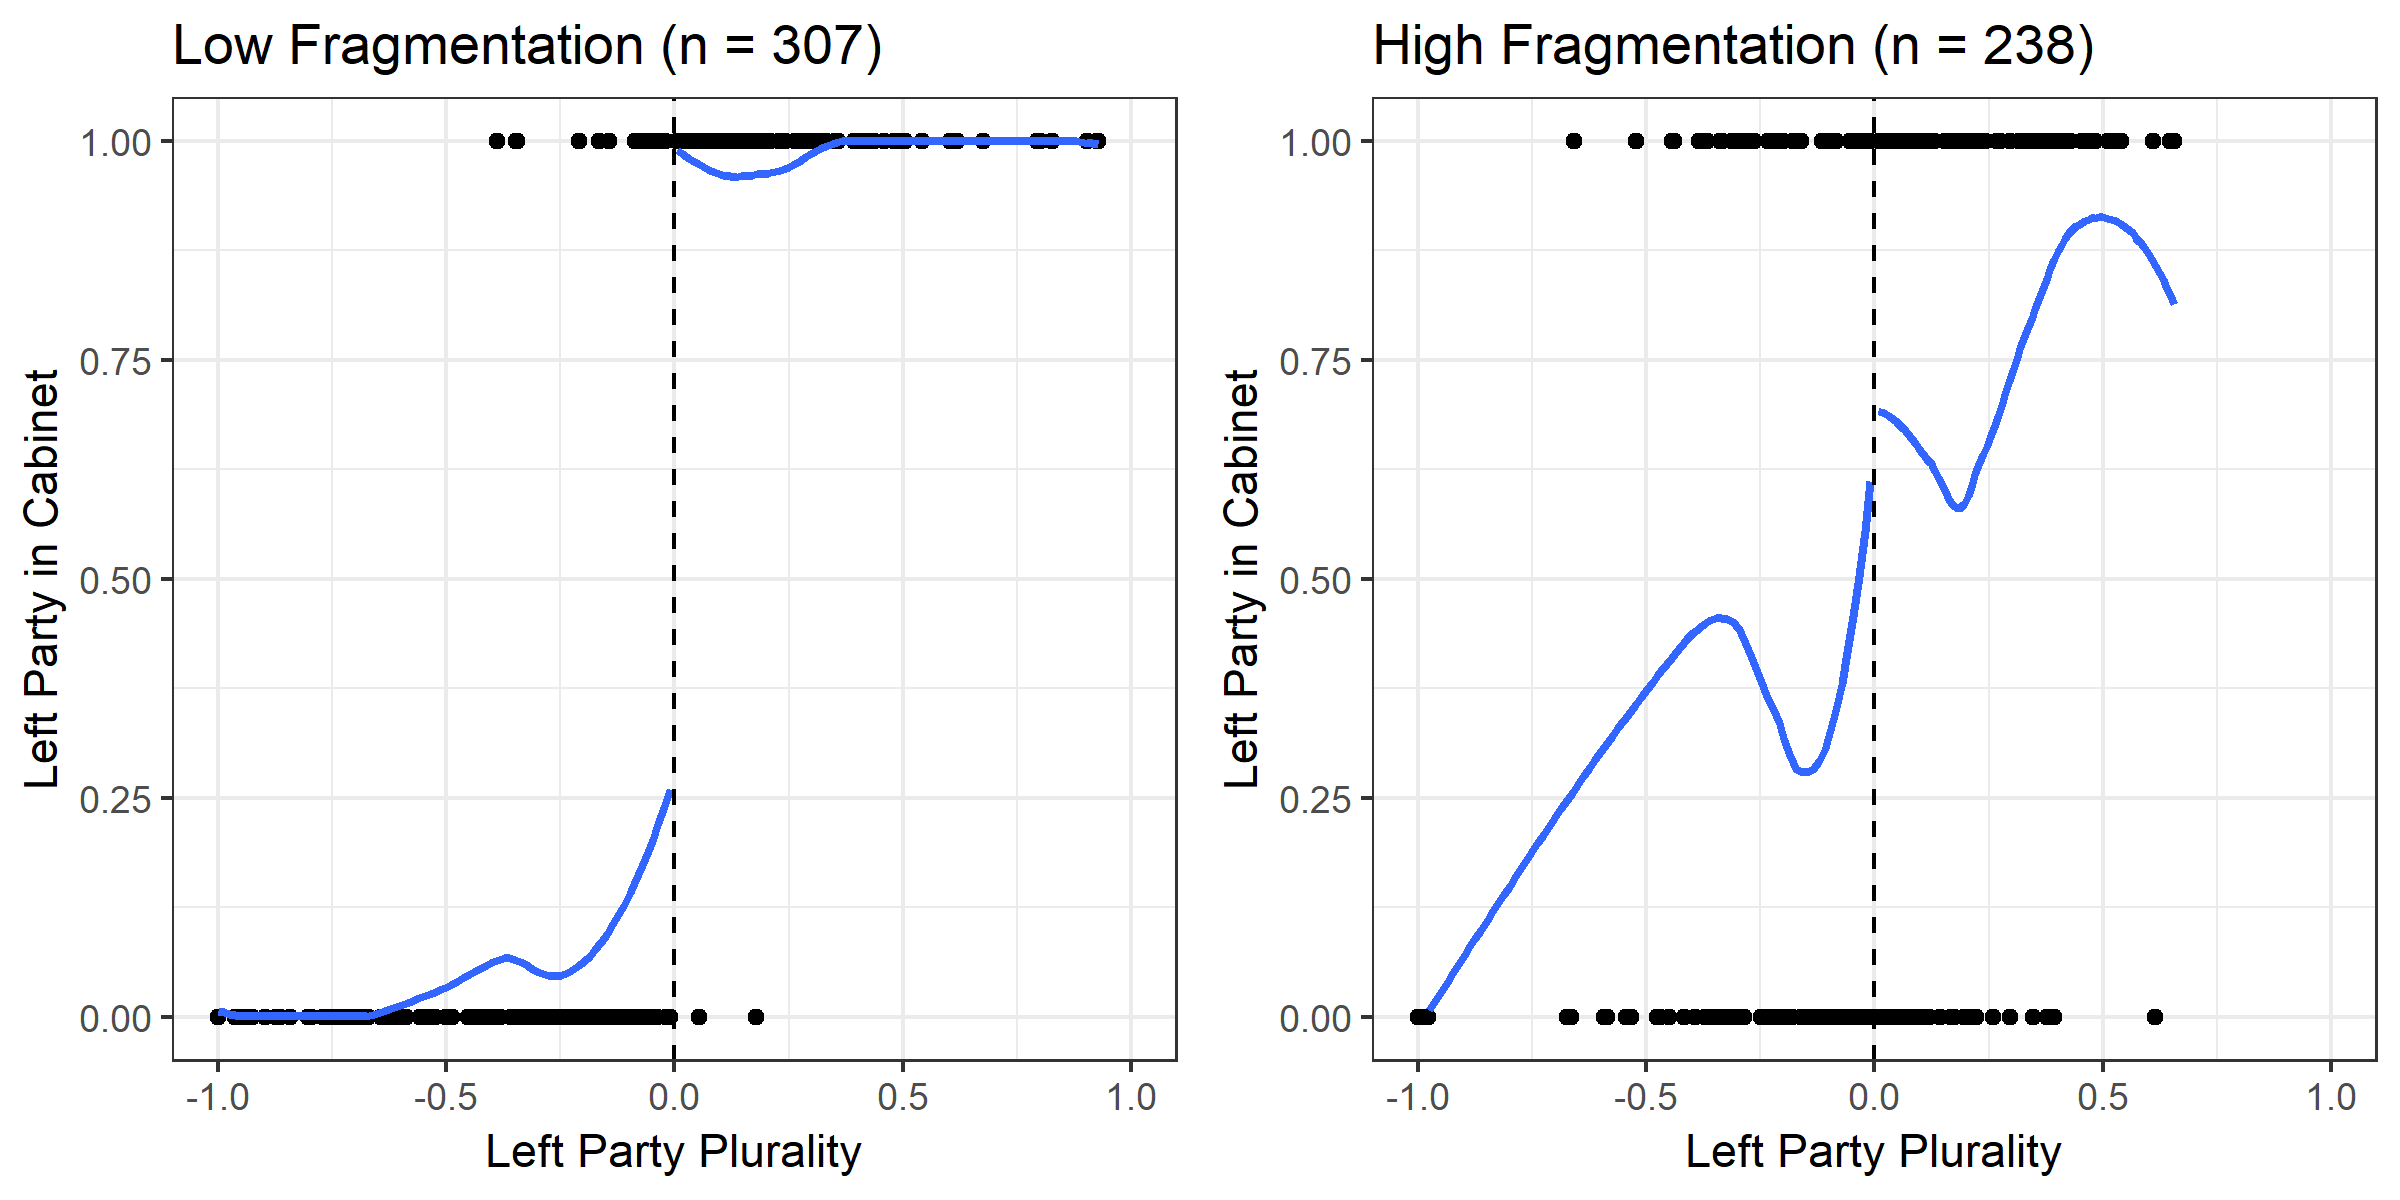
\includegraphics[width=\linewidth]{Figures/firstStageFigure}
\caption{When party fragmentation is low ($ENPP < 3.5$), there is a sharp discontinuity in the probability of left parties entering government when they achieve a plurality of seats in parliament. When party fragmentation is high ($ENPP > 3.5$), there is no such discontinuity.}
\label{fig:firststagefigure}
\end{figure}



% Table created by stargazer v.5.2.2 by Marek Hlavac, Harvard University. E-mail: hlavac at fas.harvard.edu
% Date and time: Fri, Nov 16, 2018 - 2:02:49 PM
\begin{table}[h] \centering 
  \caption{First-stage regression discontinuity estimates (bias-corrected) with 95\% confidence intervals (robust standard errors) in brackets.} 
  \label{table:firstStageRD} 
\begin{tabular}{@{\extracolsep{5pt}}lccc} 
\\[-1.8ex]\hline 
\hline \\[-1.8ex] 
 & \multicolumn{3}{c}{\textit{Fragmentation:}} \\ 
\cline{2-4} 
\\[-1.8ex] & All & Low & High \\ 
\\[-1.8ex] & (1) & (2) & (3)\\ 
\hline \\[-1.8ex] 
 Local Average Treatment Effect & 0.233 & 0.575 & 0.037 \\ 
  & [-0.035, 0.50] & [0.35, 0.80] & [-0.35, 0.42] \\ 
\hline \\[-1.8ex] 
Observations & 551 & 309 & 242 \\ 
Bandwidth Estimate $(h)$ & 0.175 & 0.218 & 0.181 \\ 
\hline 
\hline \\[-1.8ex] 
\end{tabular} 
\end{table} 


\subsection{Balance Tests}

% Paragraph 19: Balance Tests
A crucial identifying assumption for the RD design is that the treatment must be the only variable that changes discontinuously at the threshold. If any other covariates do so as well, then one cannot unequivocally attribute a discontinuity in the outcome to the treatment alone. We subject a number of pre-treatment covariates to tests of this continuity condition. For each covariate, we estimate a local-linear RD (triangular kernel), testing whether the difference in expected value on either side of the threshold differs significantly from zero. The covariates we test include GDP per capita, Polity score, population, central government debt per capita, government expenditures, tax revenue per capita, annual inflation, and OECD average bond yields. The latter test serves to ensure that our main results are not being driven by global movements in the bond market, but by country-specific bond price changes. 

% Paragraph 20: Balance Test Results
As Figure \ref{fig:balanceplots} illustrates, there are no significant discontinuities for any of these covariates, with the exception of government expenditures; elections resulting in slight left-party pluralities tend to be followed by slightly \textit{lower} central government expenditures as a percentage of GDP. Although this seems unlikely to be the cause of a discontinuity in bond yield \textit{changes}, as a robustness check we will include a variant of the RD estimator that conditions on covariates, as proposed by \citet{Calonico2018} in Appendix \ref{appendix:robustness}. These conditional-RD results are very similar to those in the primary analysis.

\begin{figure}
\centering
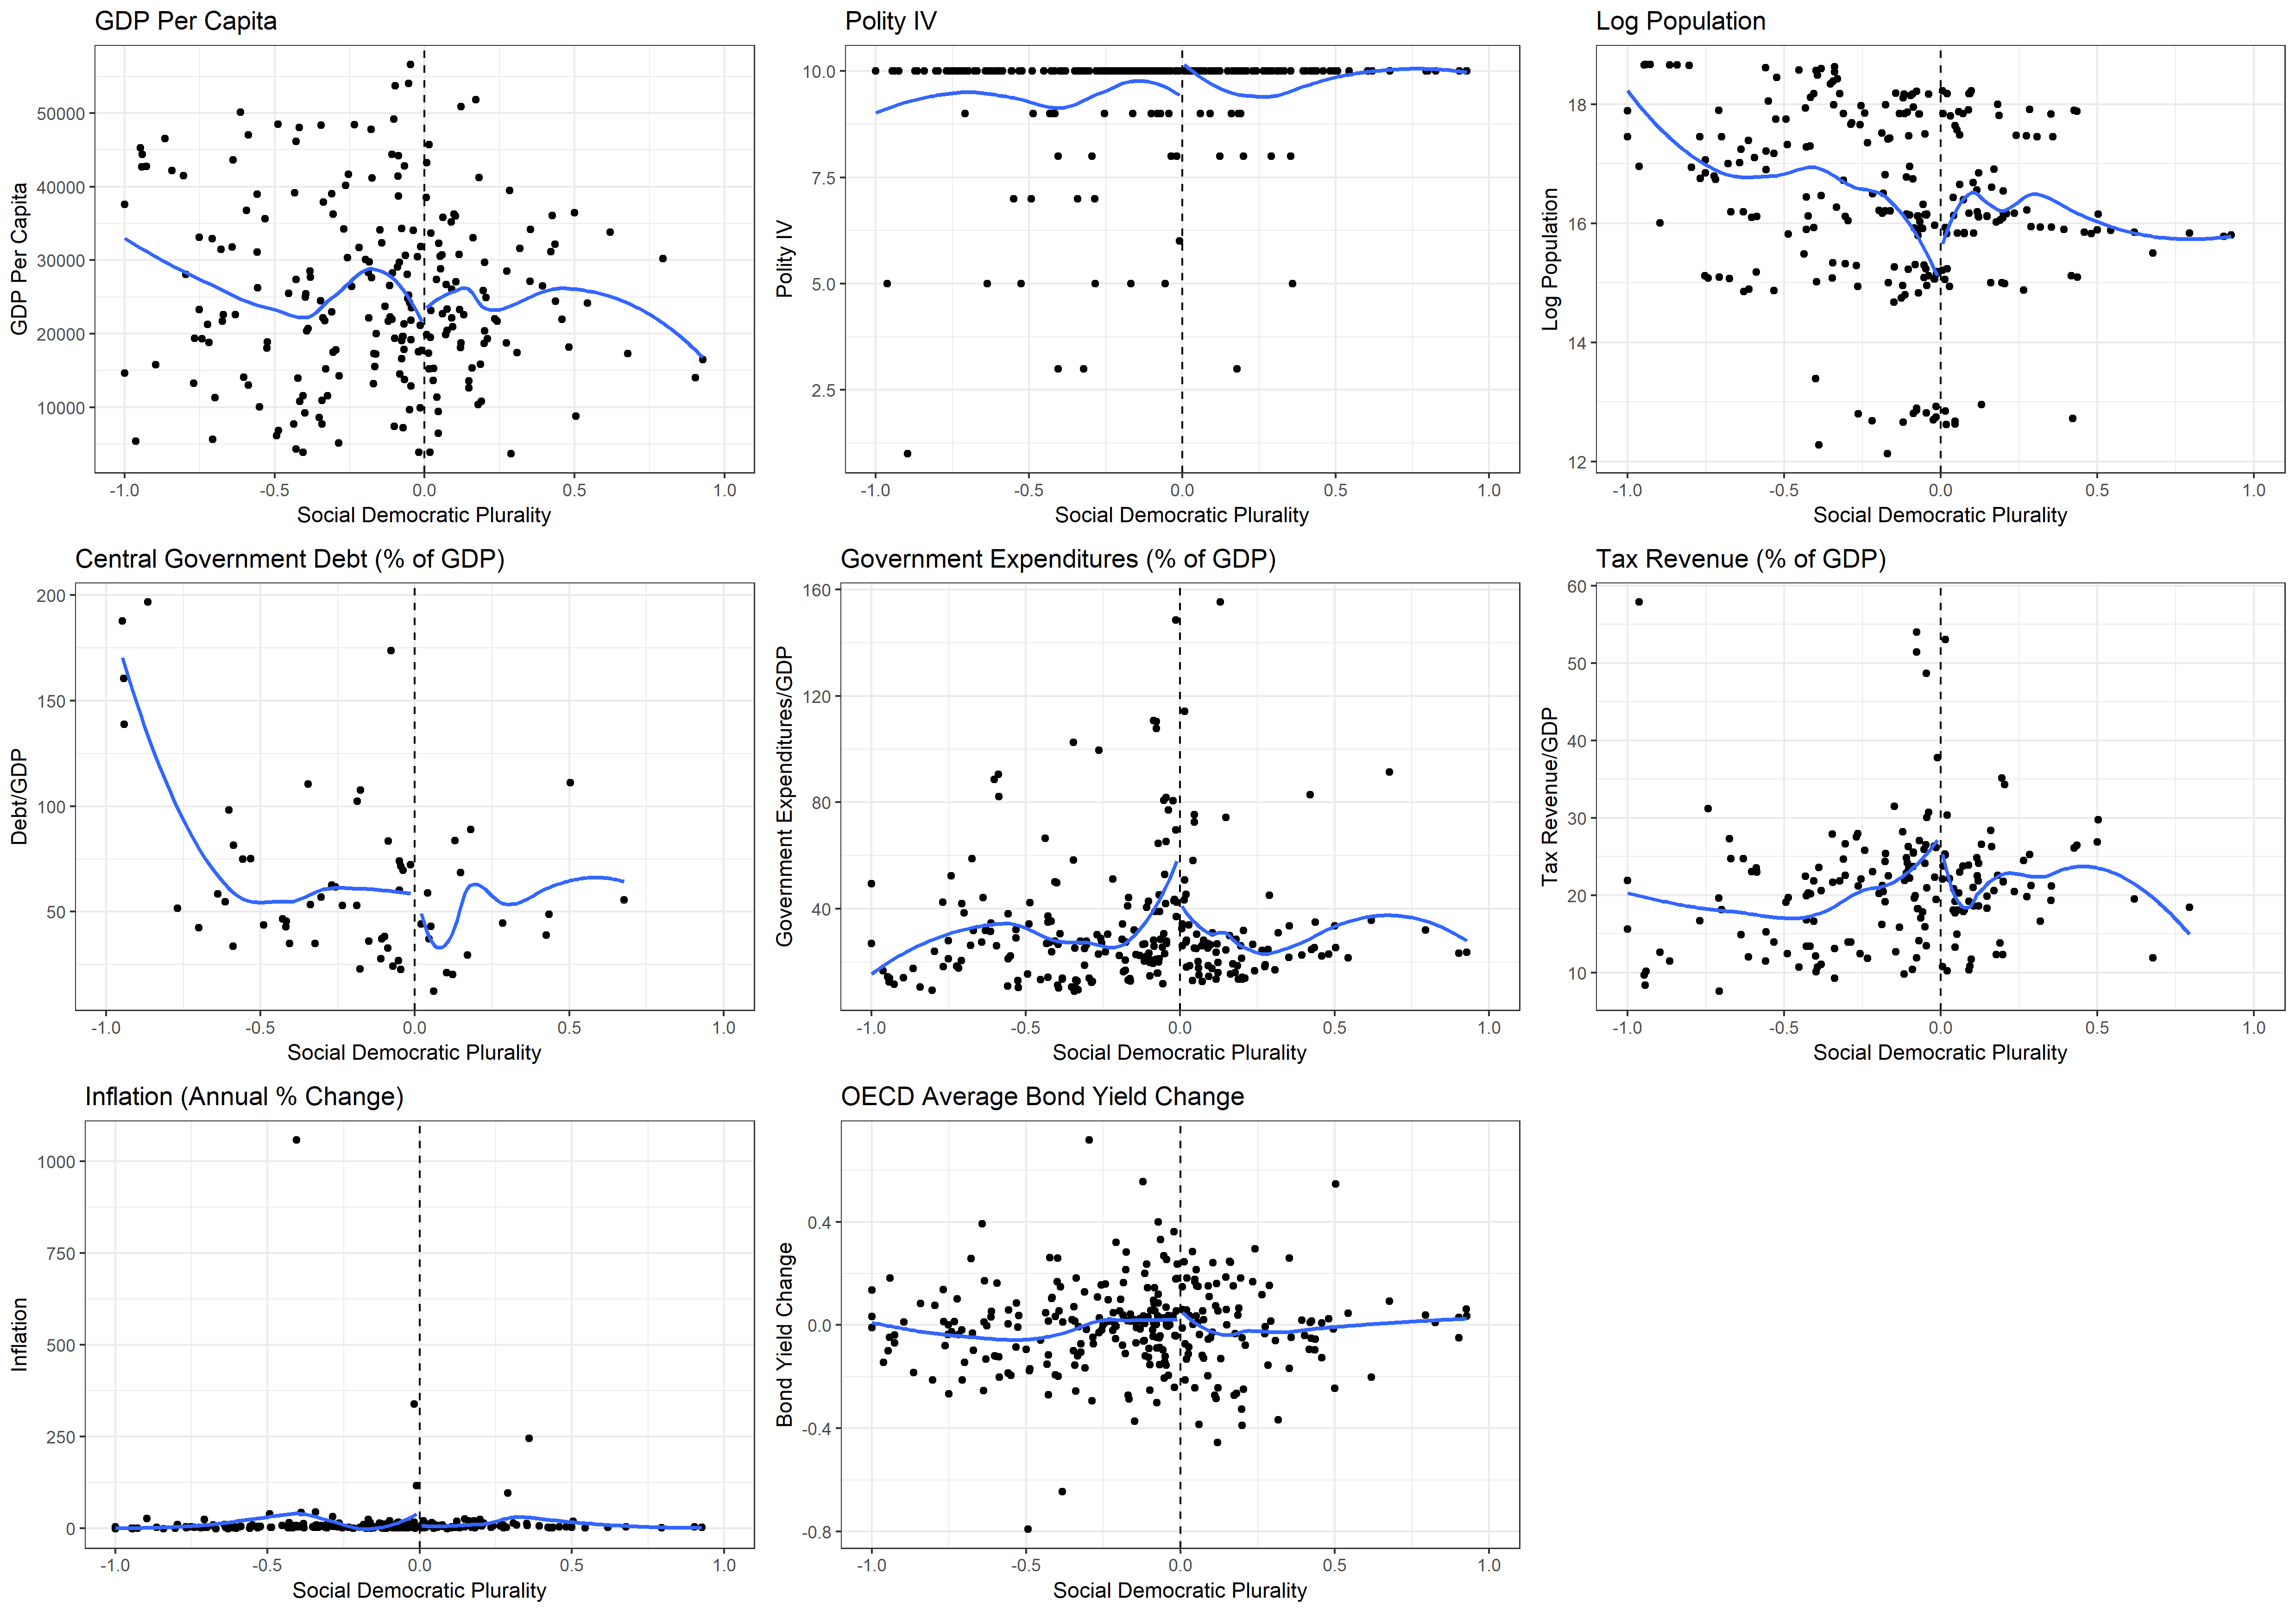
\includegraphics[width=\linewidth]{Figures/balancePlots}
\caption{For nearly every pre-treatment covariate, there is no significant discontinuity at the threshold. Note that these tests are conducted for elections with low party fragmentation, as in the primary analysis, but the finding holds when looking at the entire sample as well.}
\label{fig:balanceplots}
\end{figure}

\subsection{Bond Markets}

% Paragraph 21: LATE estimates, varying fragmentation
Table \ref{table:InterestRateRD} reports, and Figure  \ref{fig:interestraterdfigure} illustrates, the estimated Local Average Treatment Effect (LATE), in various samples according to party fragmentation. In countries with High Fragmentation ($ENPP > 3.5$), there is no statistically significant discontinuity in bond yields at the threshold. That is, left-party involvement in government does not seem to bring higher government-bond interest-premia costs in high-fragmentation contexts, perhaps because governments therein tend to be multiparty and so inertial. In contrast, in countries with Low Fragmentation ($ENPP < 3.5$), there is a roughly half-a-percentage-point increase in bond yields one month after a narrow plurality win of a left party. This is precisely what our mechanism predicts, and striking in magnitude: left-party government, at least in low-fragmentation contexts where those governments tend to be (relatively efficacious) single-party majorities, are estimated to ``cost'' roughly half a percentage point higher interest-premia on government debt! Finally, with the benefit of comparison to these low-fragmentation-sample and high-fragmentation-sample results, the entire-sample LATE estimates can be seen to have been influenced by these heterogeneous-treatment effects, to suggest only a marginally insignificant interest-rate increase less-than one-quarter as large as that in low-fragmentation contexts (and the whole-sample estimate is about 85\% noisier proportionately to effect-size).

%TODO Include num. observations within bandwidth.

% Table created by stargazer v.5.2.2 by Marek Hlavac, Harvard University. E-mail: hlavac at fas.harvard.edu
% Date and time: Fri, Nov 16, 2018 - 2:02:49 PM
\begin{table}[ht] \centering 
  \caption{1-month bond yield regression discontinuity estimates (bias-corrected) with 95\% confidence intervals (robust standard errors) in brackets.} 
  \label{table:InterestRateRD} 
\begin{tabular}{@{\extracolsep{5pt}}lccc} 
\\[-1.8ex]\hline 
\hline \\[-1.8ex] 
 & \multicolumn{3}{c}{\textit{Fragmentation:}} \\ 
\cline{2-4} 
\\[-1.8ex] & All & Low & High \\ 
\\[-1.8ex] & (1) & (2) & (3)\\ 
\hline \\[-1.8ex] 
 Local Average Treatment Effect & 0.145 & 0.592 & $-0.048$ \\ 
  & [-0.12, 0.41] & [-0.01, 1.19] & [-0.32, 0.23] \\ 
\hline \\[-1.8ex] 
Observations & 316 & 179 & 137 \\ 
Bandwidth Estimate $(h)$ & 0.137 & 0.141 & 0.125 \\ 
\hline 
\hline \\[-1.8ex] 
\end{tabular} 
\end{table}  

\begin{figure}[h]
\centering
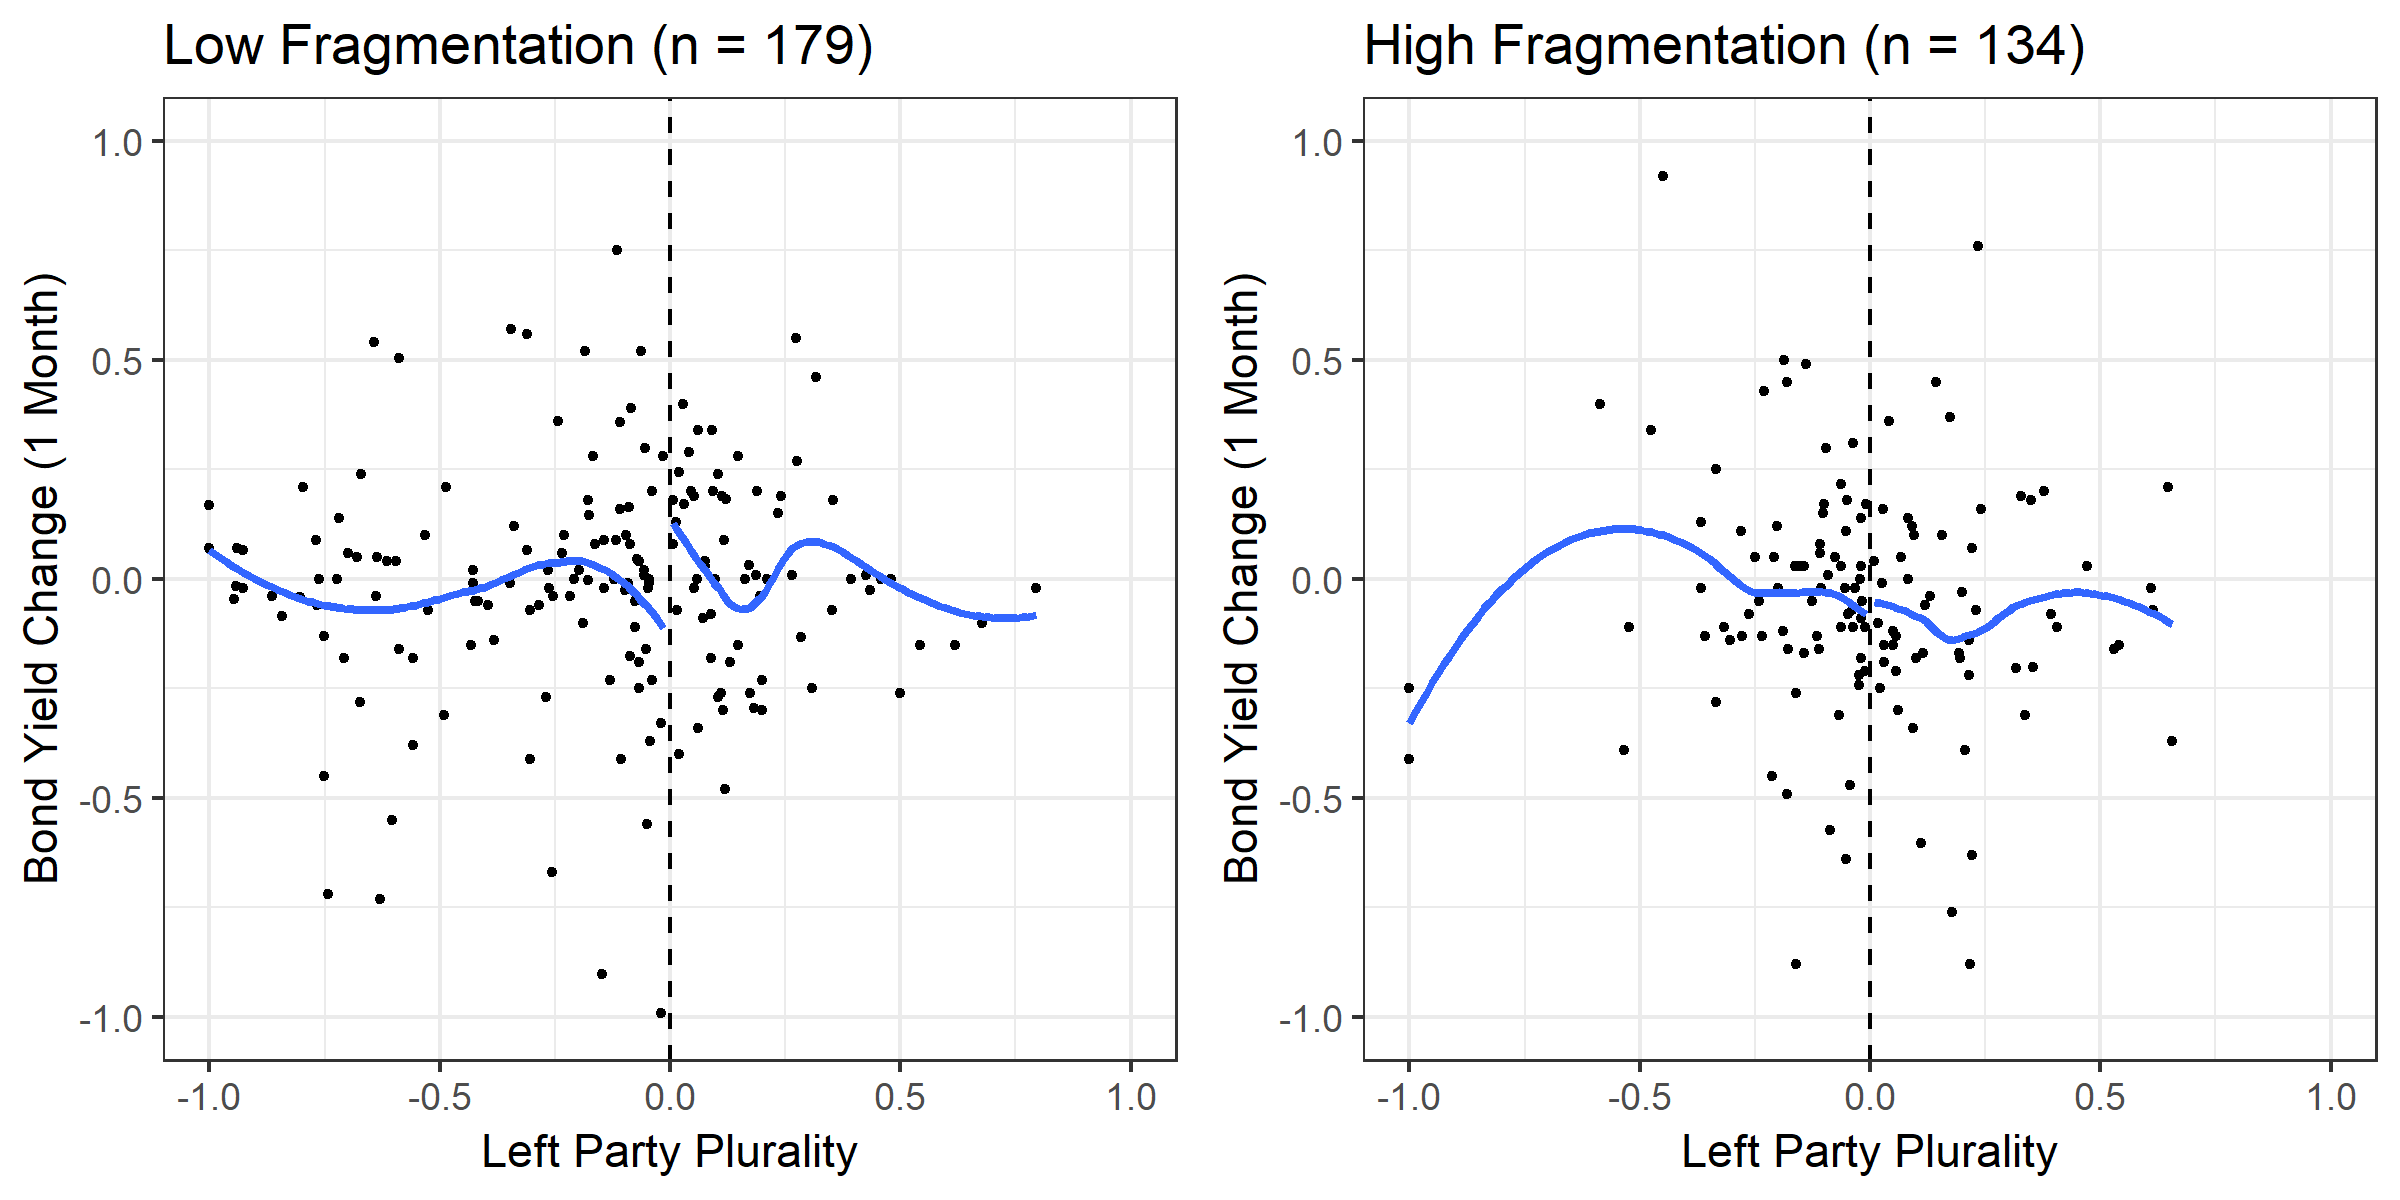
\includegraphics[width=\linewidth]{Figures/interestRateRDFigure}
\caption{Interest rate change 1 month after election, plotted against the plurality margin of the largest social democratic party.}
\label{fig:interestraterdfigure}
\end{figure}


\section{Heterogeneous Treatment Effects}

% Paragraph 22: Hetergeneous TFX 1: Ideological Distance
The strength of the bond-market response to left government likely depends on the counterfactual, namely, in this context, on how far that left government is from the alternative that \textit{would} have formed if the left had not gained the plurality. We would expect bond-market movements to be strongest when the (single) party that lost the plurality was strongly conservative relative to the (single-party) left that won. Whereas, if both parties vying for the plurality were broadly parties of the center-left, then the election outcome would have revealed little further information as financial markets would have already anticipated a center-left government of some sort, and would have priced government bonds accordingly. To explore this hypothesis, we test how the RD estimate varies with the absolute difference between the two parties' ideal points on ParlGov's ideology score.\footnote{In so doing, we are sacrificing some of the nonparametric lack of structure in our design to incorporate these \textit{measures} of ideology.} Figure \ref{fig:rdEstimateVaryingIdeologyDistance} plots these estimates. Evidence again emerges that the treatment effect arises from the information-revelation that occurs when a left party narrowly gains plurality status: the estimated effects (LATEs) are clearly larger when we restrict the sample to cases where the absolute difference in ideology score is large (e.g., greater than 3).\footnote{A caveat, however: the sample sizes for those estimates are relatively small ($n = 69$).}

\begin{figure}[h]
	\centering
	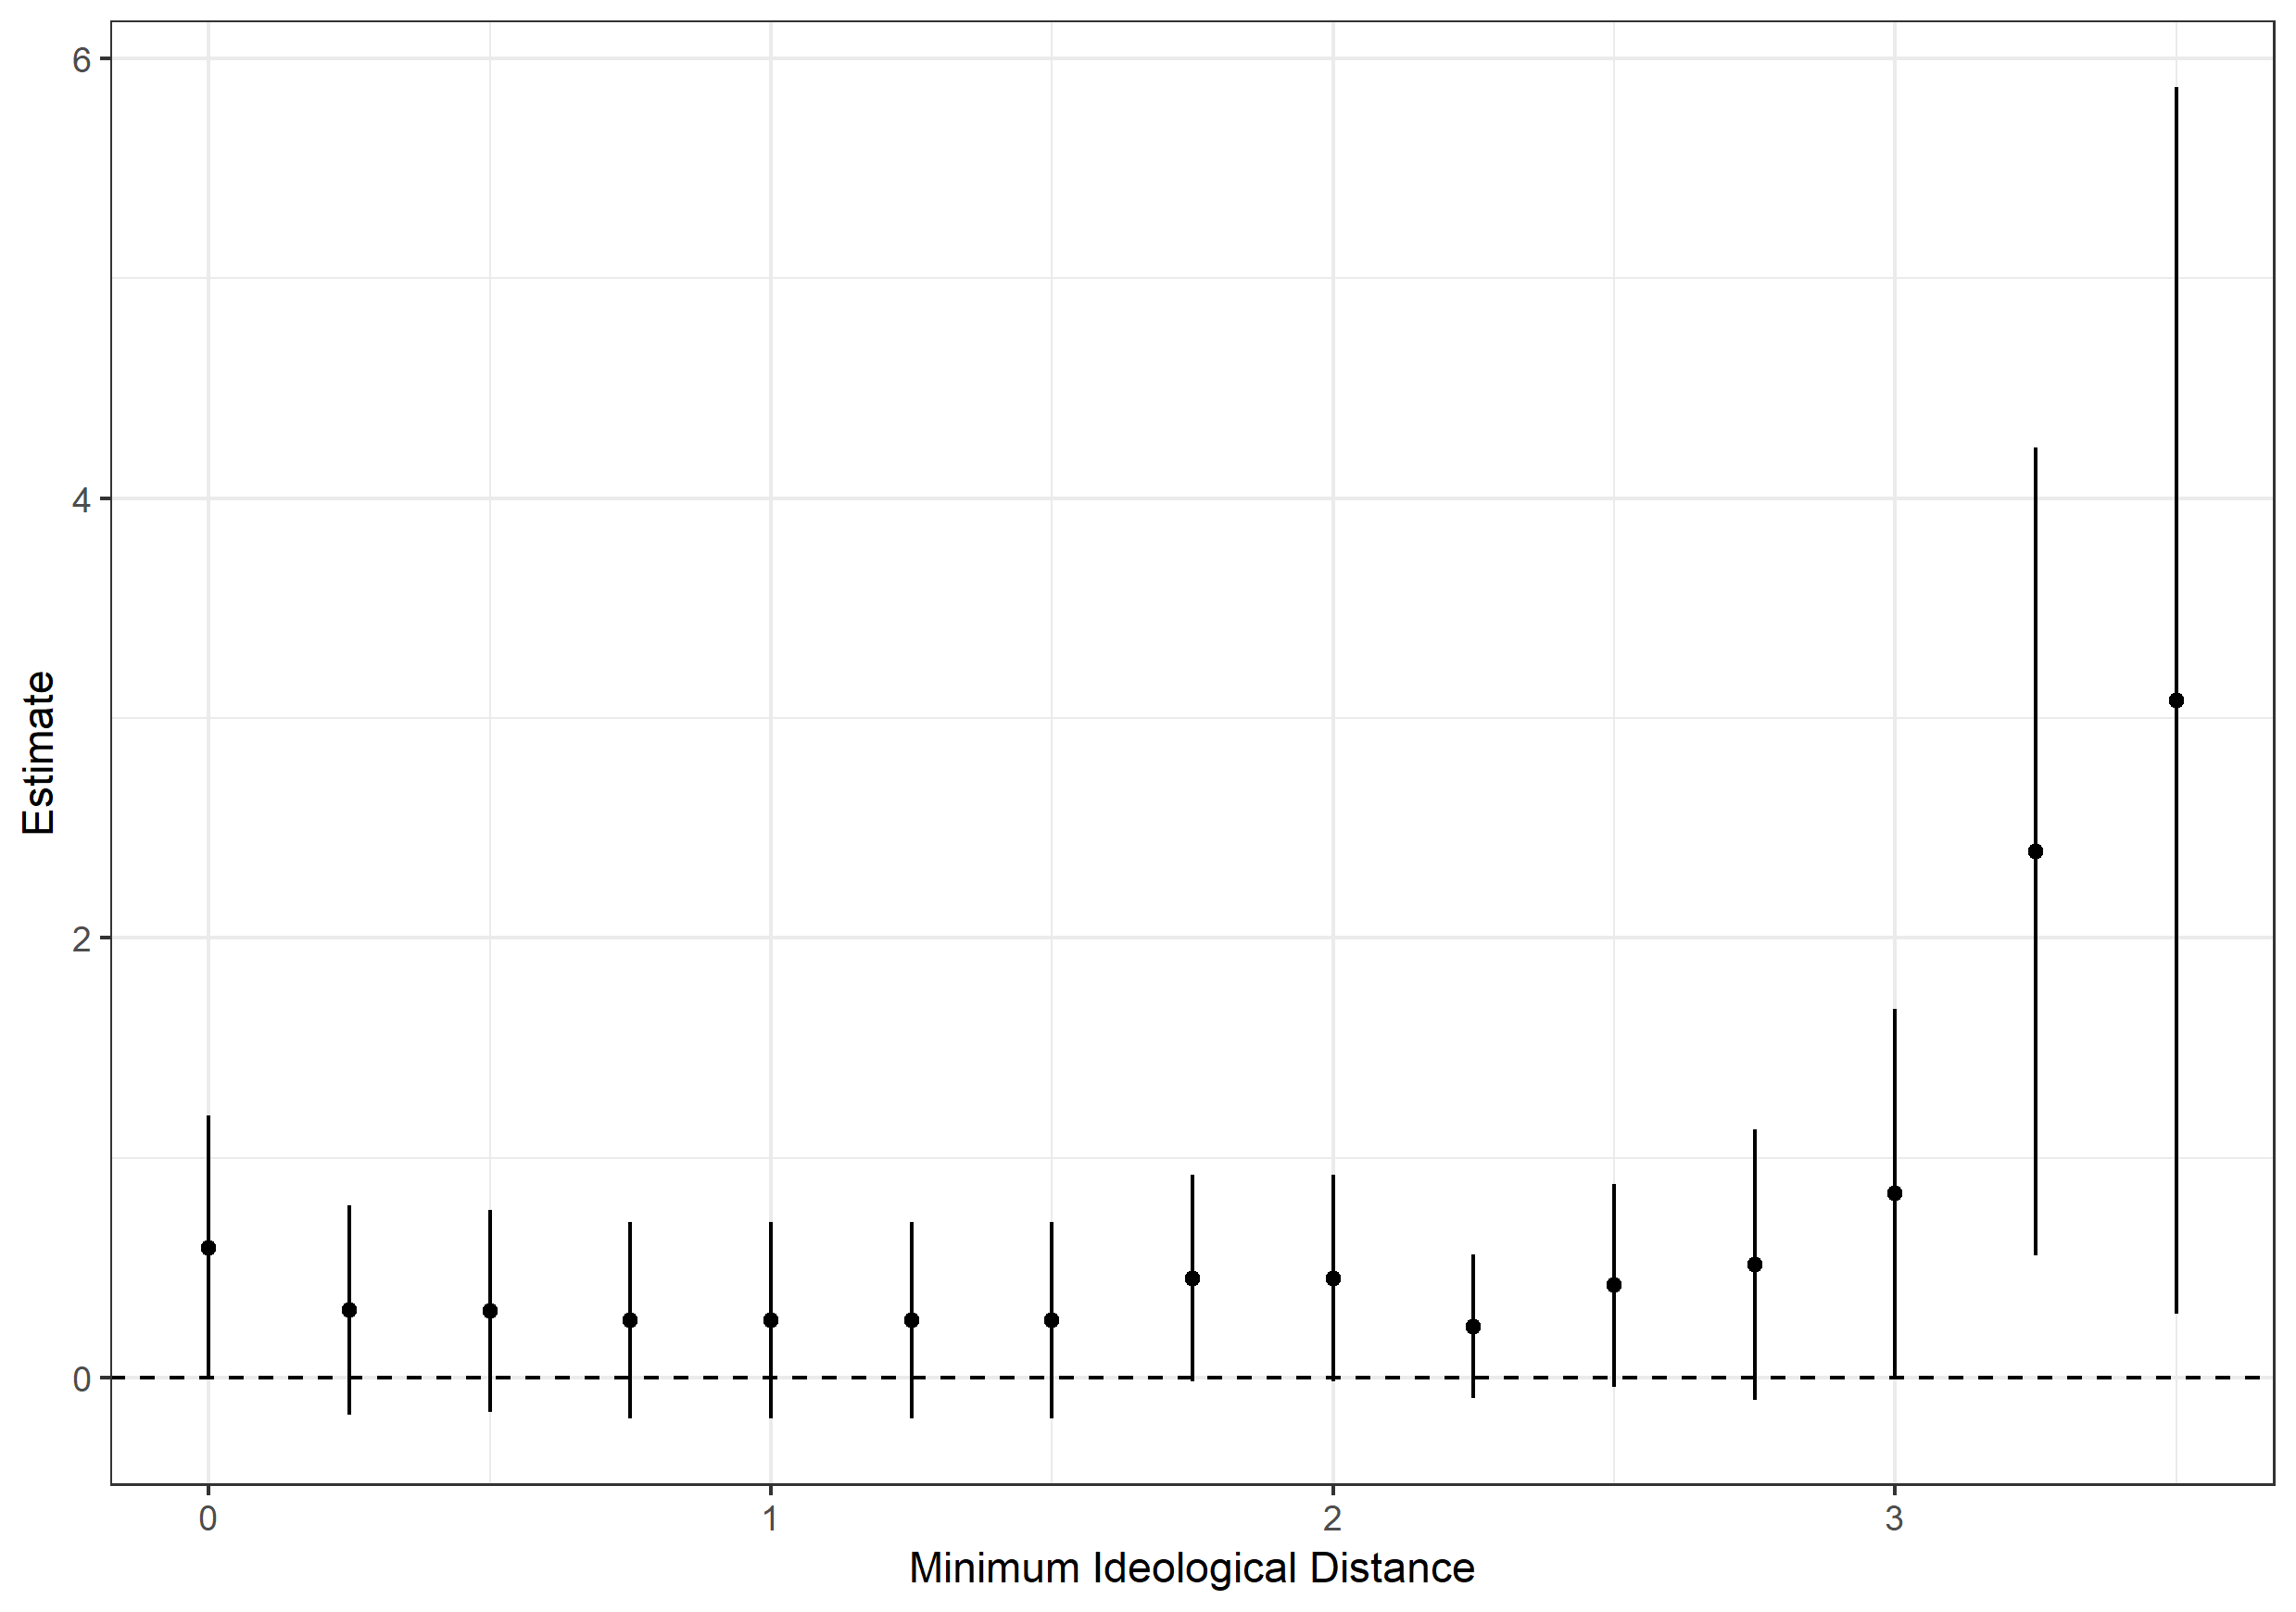
\includegraphics[width=\linewidth]{Figures/rdEstimateVaryingIdeologyDistance}
	\caption{As we restrict our estimation to elections where the two largest parties were far apart from one another in ideological distance, the estimated treatment effect grows.}
	\label{fig:rdEstimateVaryingIdeologyDistance}
\end{figure}

% Paragraph 23: Heterogeneous TFX 2: Historical Era
Finally, Figure \ref{fig:rdEstimateVaryingYear} illustrates how the estimated effect varies over time -- each point reports an estimate and confidence interval from a 30-year window of data starting from the year indicated on the X-axis. Interestingly, it is around the Bretton Woods era of fixed exchange-rates and low capital-mobility (approximately from the early 1950s through the mid-to-late 1970s) that the interest-rate effect of left government is largest and most discernible. This would be consistent with Rodrik's ``golden straightjacket'' hypothesis -- i.e., with considerable globalization-and-capital-mobility constraint on domestic governments' policymaking autonomy, \textit{if} it is also the case that the reason we are not finding interest-rate effects of left government is because their policies do not (or are not expected to) differ much from other governments in this later period. After all, furthermore, Mundell-Fleming suggests that monetary and fiscal policy should have been at least moderately maneuverable and effective in that 1950s-1970s era of limited capital-mobility and \textit{imperfectly} fixed exchange-rates; and both monetary and fiscal policy should have grown less maneuverable and/or effective, even though exchange-rate-fixing efforts lessened at least initially for a time, as capital grew highly mobile and the remaining dependent central banks increasingly independent \citep{Clark2003, Franzese2003}.

\begin{figure}
\centering
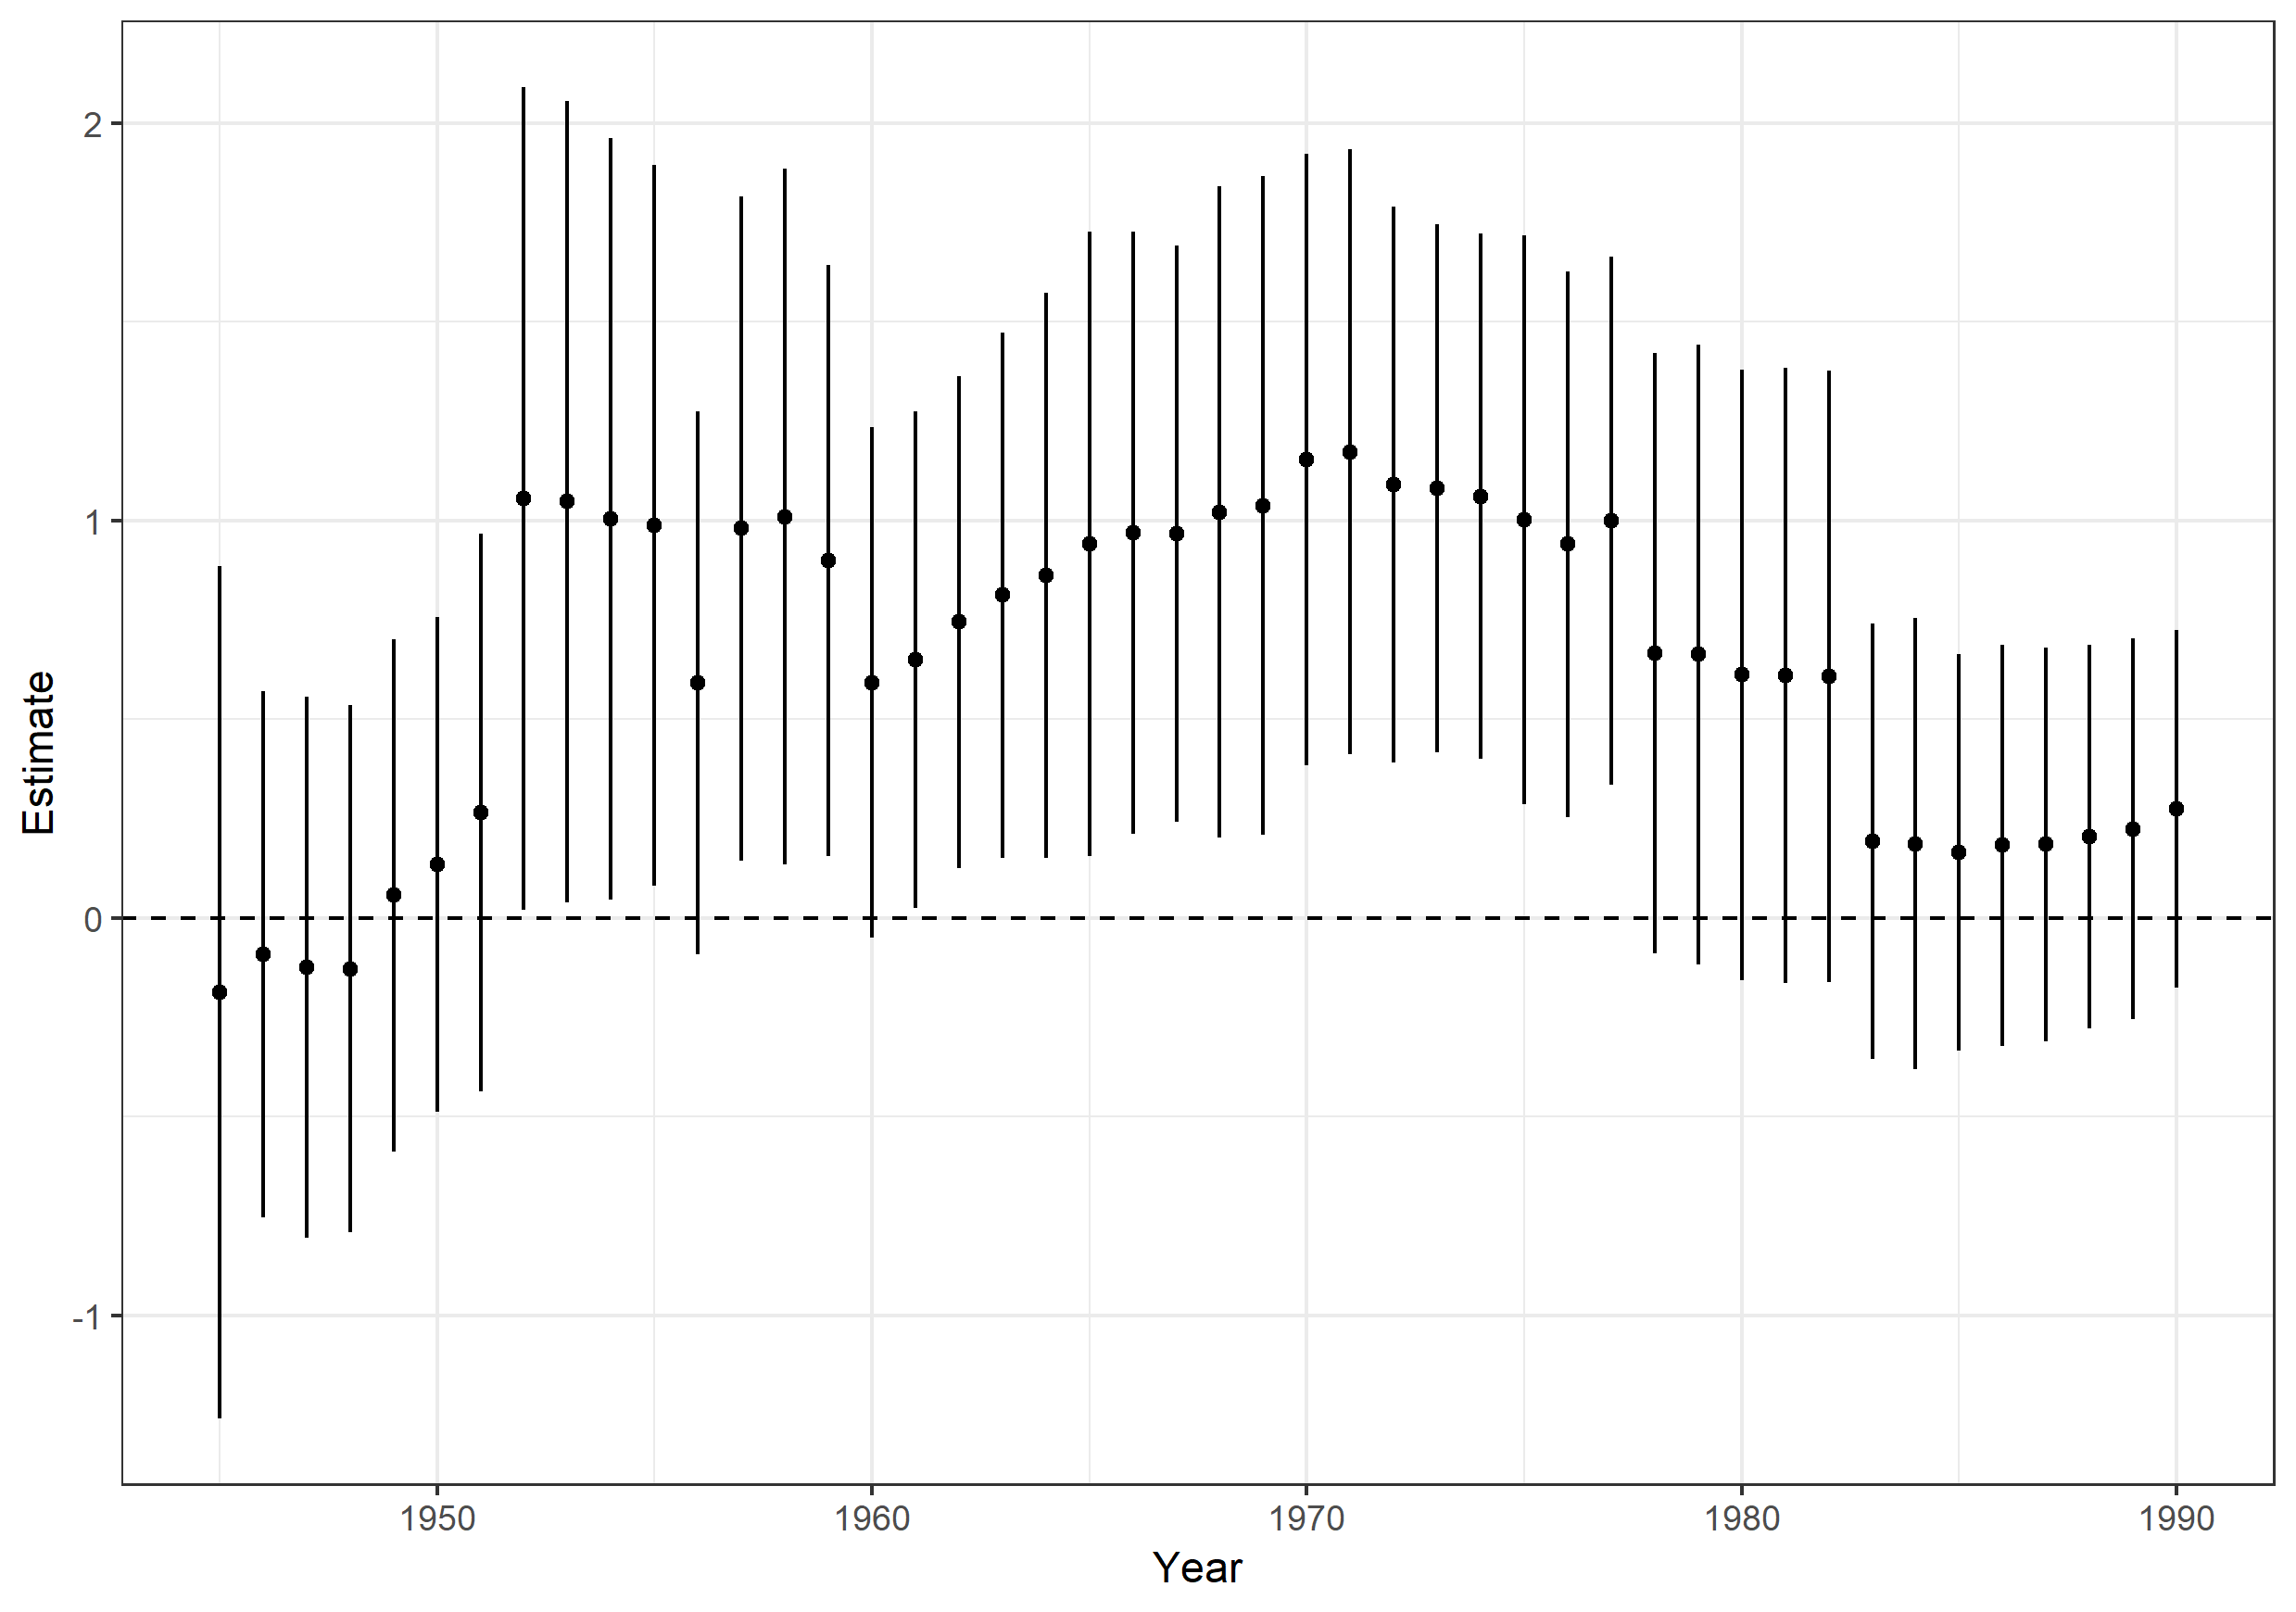
\includegraphics[width=\linewidth]{Figures/rdEstimateVaryingYear}
\caption{RD estimates and 95\% confidence intervals, varying the time period of analysis. (Each point is estimated using 30 years of data; x-axis denotes the minimum year.)}
\label{fig:rdEstimateVaryingYear}
\end{figure}

\section{Conclusion}

% Paragraph 24: Summarize Results
A discontinuous increase in the probability of government entry at the  parliamentary-seat plurality threshold offers quasi-experimental identification of the causal effect, in that plurality-threshold vicinity, of that party on outcomes we think the party may influence in government. We focused on the interest-rate-premium cost of left-party government that financial markets add to government-bond yields. Applying a regression discontinuity design to this core question of the (interest-rate) ``cost of left government'', and varying refinements of the question, we were able to estimate that left government indeed carries quite sizable interest-rate costs, over 0.5 percentage points, in the short term -- for around a year or a little more, peaking at around 10 months -- under certain conditions, namely when party-system fragmentation is low, so that (we suspect) government alternation tends to be between relative distant left and right single-party-majority alternatives. Contrarily, such clearly discernible and appreciable interest-rate effects do not seem to materialize in more-fragmented party-system contexts, we suspect because in those contexts government alternation is not as stark in ideological-distance terms and bare-plurality left parties there tend to be entering multiparty coalition and/or minority, and so more inertial, governments. Also, we found that the time window in which these notable interest-rate costs of left governments in low-fragmentation systems arose was furthermore limited to a period around the Bretton Woods era from the early 1950s through the mid-to-late 1970s in which capital mobility was limited and exchange rates were imperfectly fixed (among our sample countries, \textit{de facto}, to the (extra-sample) U.S. dollar). Under the conditions prevailing in this window, autonomous domestic government monetary and fiscal policy maneuverability and efficacy would have been reasonably high. As these (and other: e.g., high and rising central-bank independence) conditions changed, domestic-government policymaking autonomy, maneuverability, and efficacy will have faded, which could explain the reduced magnitude and certainty of left interest-rate cost we estimate in these later periods. To explore how accurate are our interpretations of the varying interest-rate costs of left government that we estimated in low-fragmentation \textit{versus} high-fragmentation contexts, and across the moving-window estimates showing sizable and discernible effects only in the 1950s through 1970s period, future analyses should explore macroeconomic-policy differences near the discontinuity. Are there differences in policy that could explain the variation in the estimated interest-premium effects corresponding to differences in domestic and international political-economic institutions and structure that we suggest are driving these heterogeneous effects we discovered. \textit{Inter alia}, these analyses will help distinguish whether we observe Downsian convergence in policies due to democratic competition and so in financial-market outcomes; convergence in policies and outcomes from globalization-induced policy competition; convergence in outcomes but not policy indicating lack of market concern about those policies or suggesting some non-policy-related market reaction to left government; and/or some other political-economic institutional-contextual conditioning of partisan-government effects on policy and/or outcomes that could be driving these varying interest-premium costs of left government.

% Paragraph 25: Limitations and Future Work
There are a couple of important limitations and potential pitfalls to the approach we are proposing. One obvious problem stems from the fact we are relying on an \textit{ex post} measure of \textit{ex ante} uncertainty. Or, more exactly, we are using an \textit{ex post} measure of how uncertain the election outcome was--how close to 50-50 was the proposition of left-party being largest--whereas the actually relevant concept for market reaction is how surprisingly left was the government. In order to construct a true \textit{ex ante} measure of government-partisanship surprise, we would need pre-election polls (which are not available on the scale we require), party partisanship measures, and some manner of translating government-party partisanship to government partisanship--and each of these components would furthermore require structural specifications. Unfortunately, this is the best that can be done (especially insofar as we wish to retain non-parametric causal-inference robustness over structural-specification efficiency). However, we are confident that the \textit{ex post} measure of electoral uncertainty is unbiased with respect to \textit{ex ante} electoral uncertainty at least. Some elections that are forecasted to be close are landslides and some landslides are predicted to be close, but these occurrences are rare and random. Another limitation stems from the small number of close elections. Although we counted 95 close elections -- defined as top left-right parties' seat-differential of $\pm$10\% so that a 5\% swing would have switched the winner -- in parliamentary democracies from 1948-2015, we have data on bond yields for only forty-nine of these close-election contexts. Notwithstanding this relatively small pool for comparing interest rates in left near-losses to left close-wins, the sample-size may prove adequate given that market reactions are theorized to be the largest at the threshold. Even so, this caveat is worthwhile warning to remember when interpreting the results that power may be an issue. Finally, we must pool countries with widely disparate institutions and draw cases from an extended historical period. Although this kind of pooling is common practice in comparative political economy (e.g., \citet{Beck1995}), it comes with complications that are worth keeping in mind. For example, pooling majoritarian and proportional parliamentary democracies may mask other differences because the former tend to produce single-party left and right governments for comparison on either side of the threshold whereas the latter tend to produce coalition governments on both sides. This particular potential heterogeneity in treatments will be probed below, but others are likely across this wide diversity of parliamentary democracies. Unaccounted treatment heterogeneity, akin to specification error, induces inefficiency at best (if the heterogeneity is unrelated to treatment) and bias at worst (if related).

\bibliography{refs}


\begin{appendices}
	
	
	\section{Robustness Tests} \label{appendix:robustness}
	
	\subsection{Varying the ENPP Threshold}
    
    Figure \ref{fig:LowFragHighFrag} plots party fragmentation -- measured by ENPP -- for each country-year in our dataset. As the figure makes clear, the Low Fragmentation countries are not exclusively majoritarian single-party governments. They include countries with proportional representation, like Spain and Portugal, and countries with frequent coalition governments, like Germany.
    
    \begin{figure}[h]
		\centering
		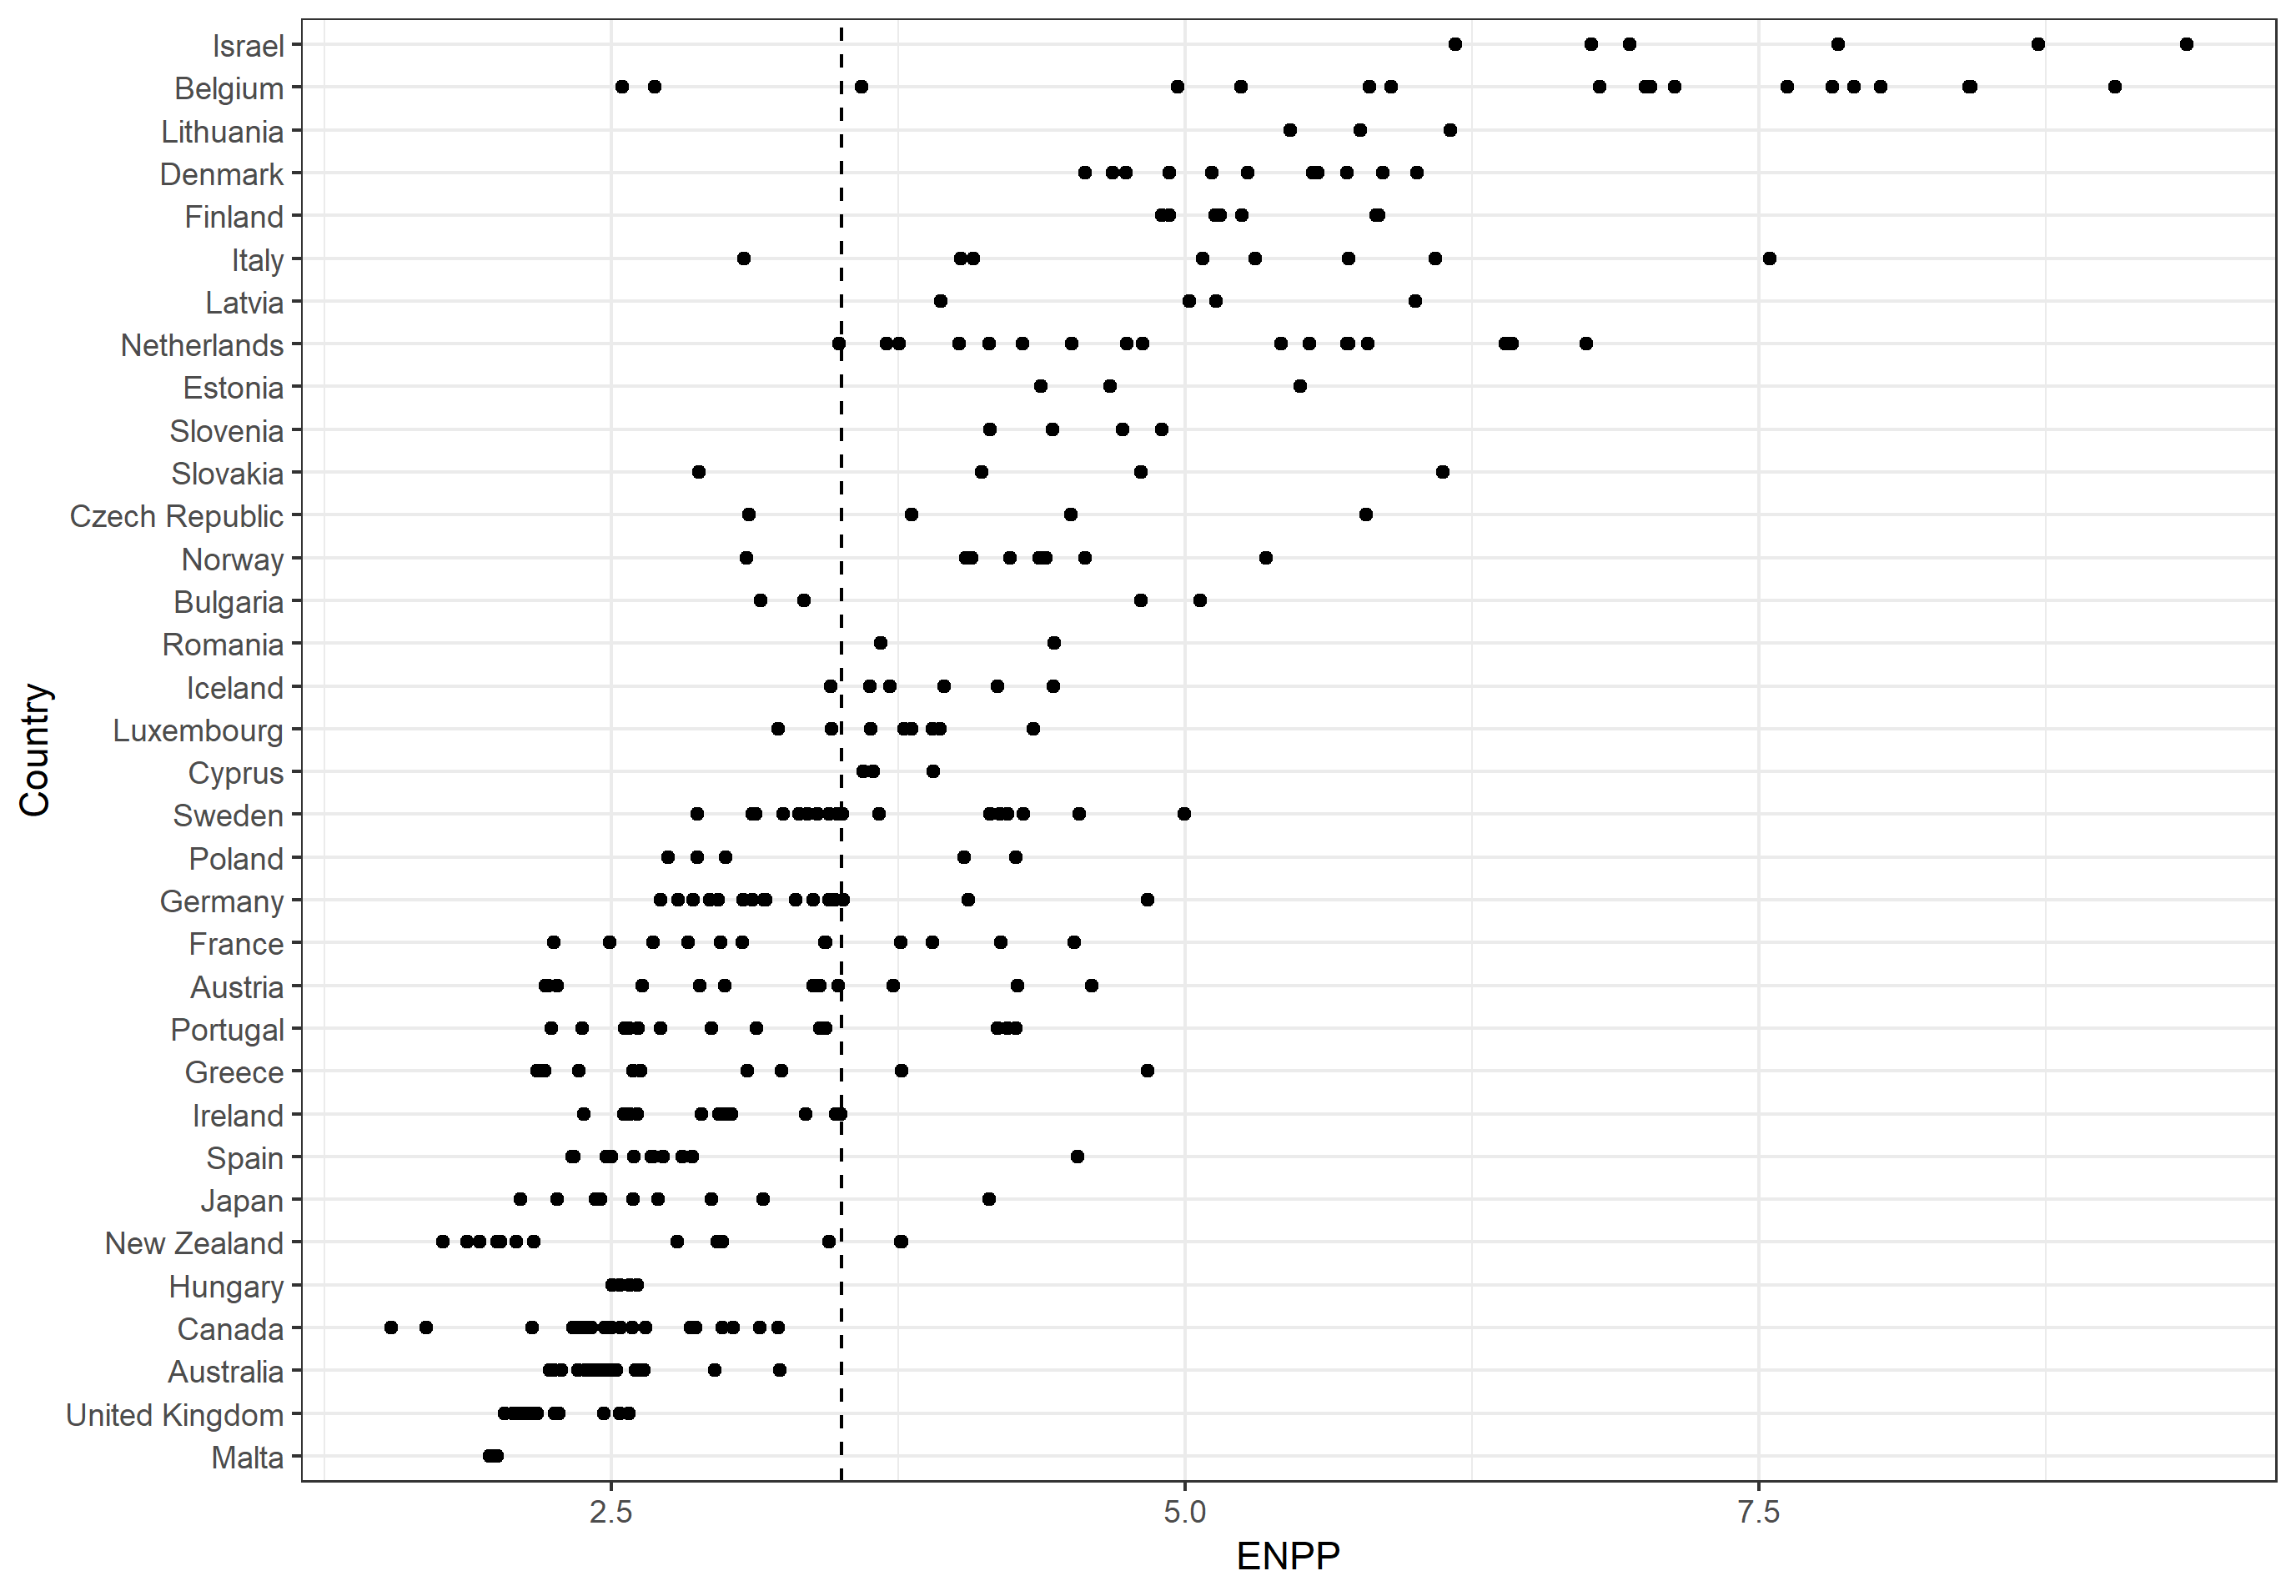
\includegraphics[width=\linewidth]{Figures/LowFragHighFrag.png}
		\caption{Party fragmentation in parliament by country-year. The dashed vertical line is our cutoff for classifying low vs. high fragmentation elections.}
		\label{fig:LowFragHighFrag}
	\end{figure}
    
	Figure \ref{fig:rdEstimateVaryingENPP} illustrates how the RD estimate and 95\% confidence interval changes when we vary the ENPP threshold. The result holds for cutoffs less than 3.5, though when it is less than 3 the effective sample size is much smaller, yielding larger robust standard errors. 
	
	\begin{figure}[h]
		\centering
		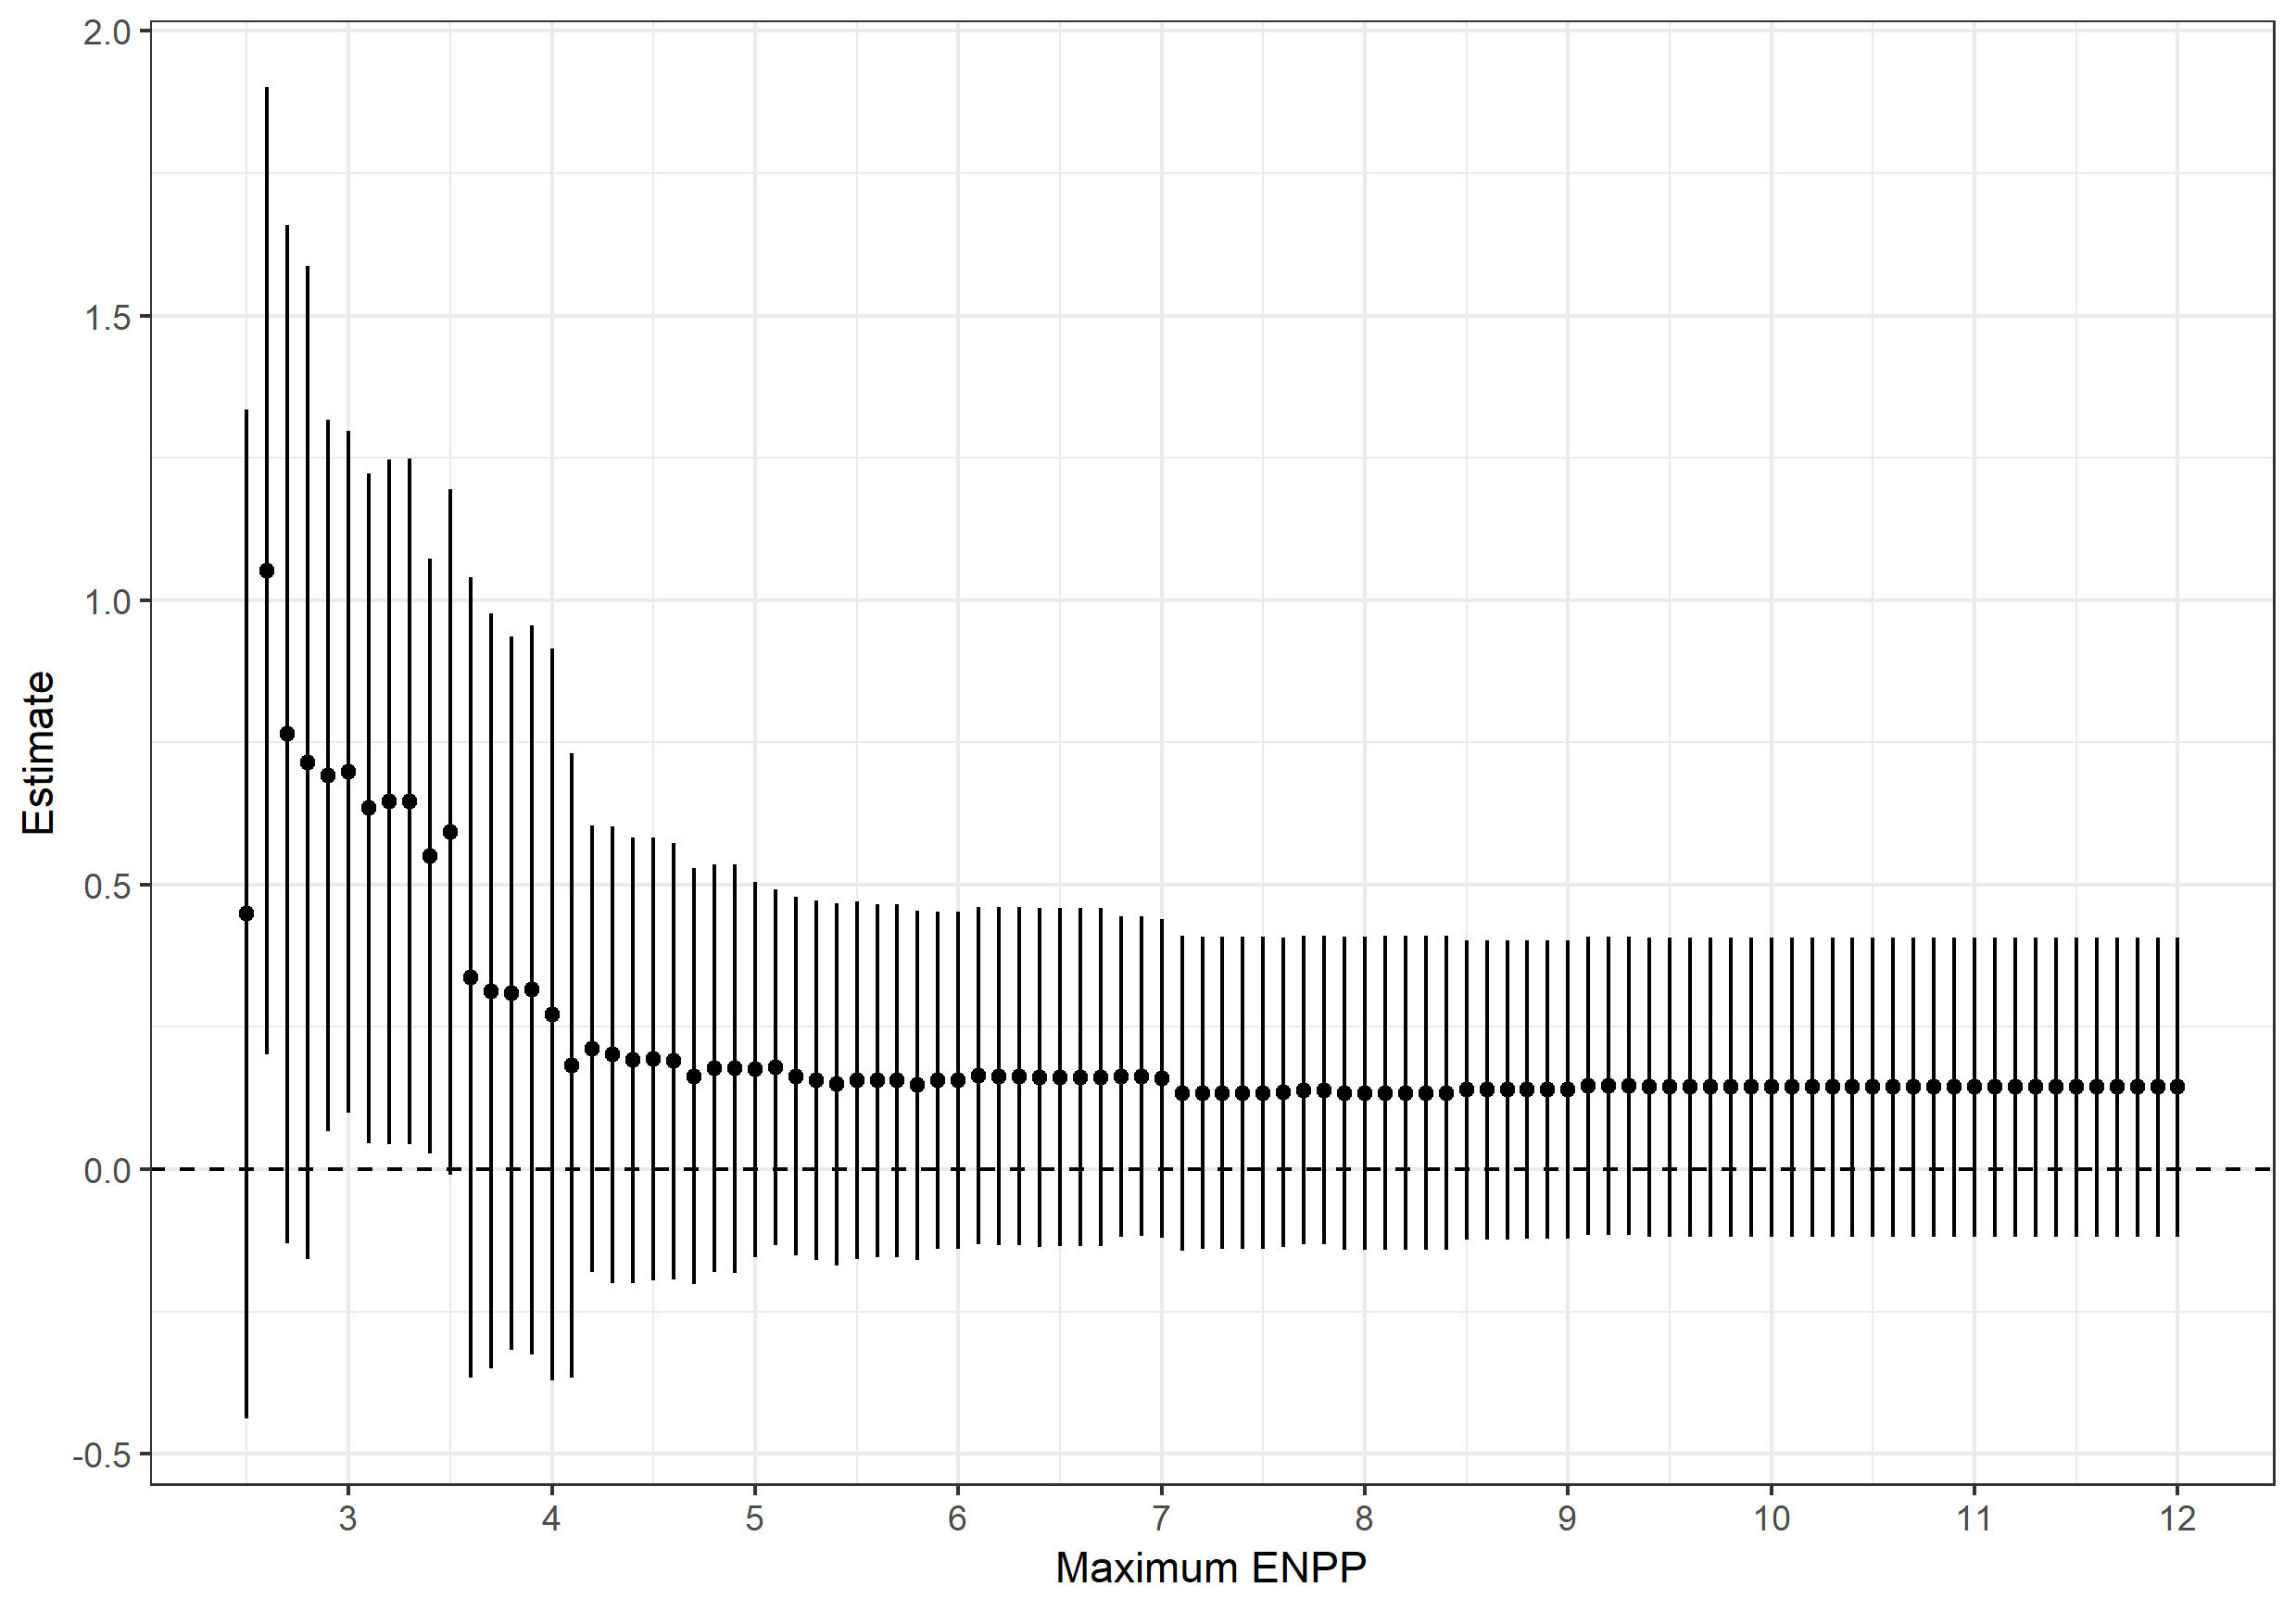
\includegraphics[width=\linewidth]{Figures/rdEstimateVaryingENPP}
		\caption{Estimated treatment effects and 95\% confidence intervals, varying the ENPP threshold. The estimate is largest when party fragmentation is low (ENPP $< 3.5$)}
		\label{fig:rdEstimateVaryingENPP}
	\end{figure}

	\subsection{Regression Discontinuity with Covariates}
	
	\citet{Calonico2018} propose a procedure to adjust for covariates in a regression discontinuity framework. Estimating using this procedure -- conditioning on GDP per capita, log population, expenditures per capita, tax revenue as a percentage of GDP, and inflation -- yields the results in Table \ref{table:RDWithCovariates}. 
	
	% Table created by stargazer v.5.2.2 by Marek Hlavac, Harvard University. E-mail: hlavac at fas.harvard.edu
	% Date and time: Fri, Nov 16, 2018 - 2:02:49 PM
	\begin{table}[h] \centering 
		\caption{Regression discontinuity with pre-treatment covariates. Dependent variable = 1-month bond yield regression discontinuity estimates (bias-corrected) with 95\% confidence intervals (robust standard errors) in brackets.} 
		\label{table:RDWithCovariates} 
		\begin{tabular}{@{\extracolsep{5pt}}lccc} 
			\\[-1.8ex]\hline 
			\hline \\[-1.8ex] 
			& \multicolumn{3}{c}{\textit{Fragmentation:}} \\ 
			\cline{2-4} 
			\\[-1.8ex] & All & Low & High \\ 
			\\[-1.8ex] & (1) & (2) & (3)\\ 
			\hline \\[-1.8ex] 
			Local Average Treatment Effect & 0.146 & 1.01 & $-0.146$ \\ 
			& [-0.14, 0.43] & [0.46, 1.56] & [-0.45, 0.16] \\ 
			\hline \\[-1.8ex] 
			Observations & 236 & 118 & 118 \\ 
			Bandwidth Estimate $(h)$ & 0.138 & 0.135 & 0.129 \\ 
			\hline 
			\hline \\[-1.8ex] 
		\end{tabular} 
	\end{table}  


	\subsection{Sensitivity to Bandwidth}
	
	As Figure \ref{fig:bandwidthSensitivity} illustrates, our result is somewhat sensitive to choice of bandwidth. Using a smaller bandwidth than the CCT optimum yields significantly fewer observations near the cutoff, increasing standard errors. And the local-linear estimate shrinks with larger bandwidths (as would be expected, given the theoretical conditional expectation function \ref{section:design}.) 
	
	
	\begin{figure}[h]
	\centering
	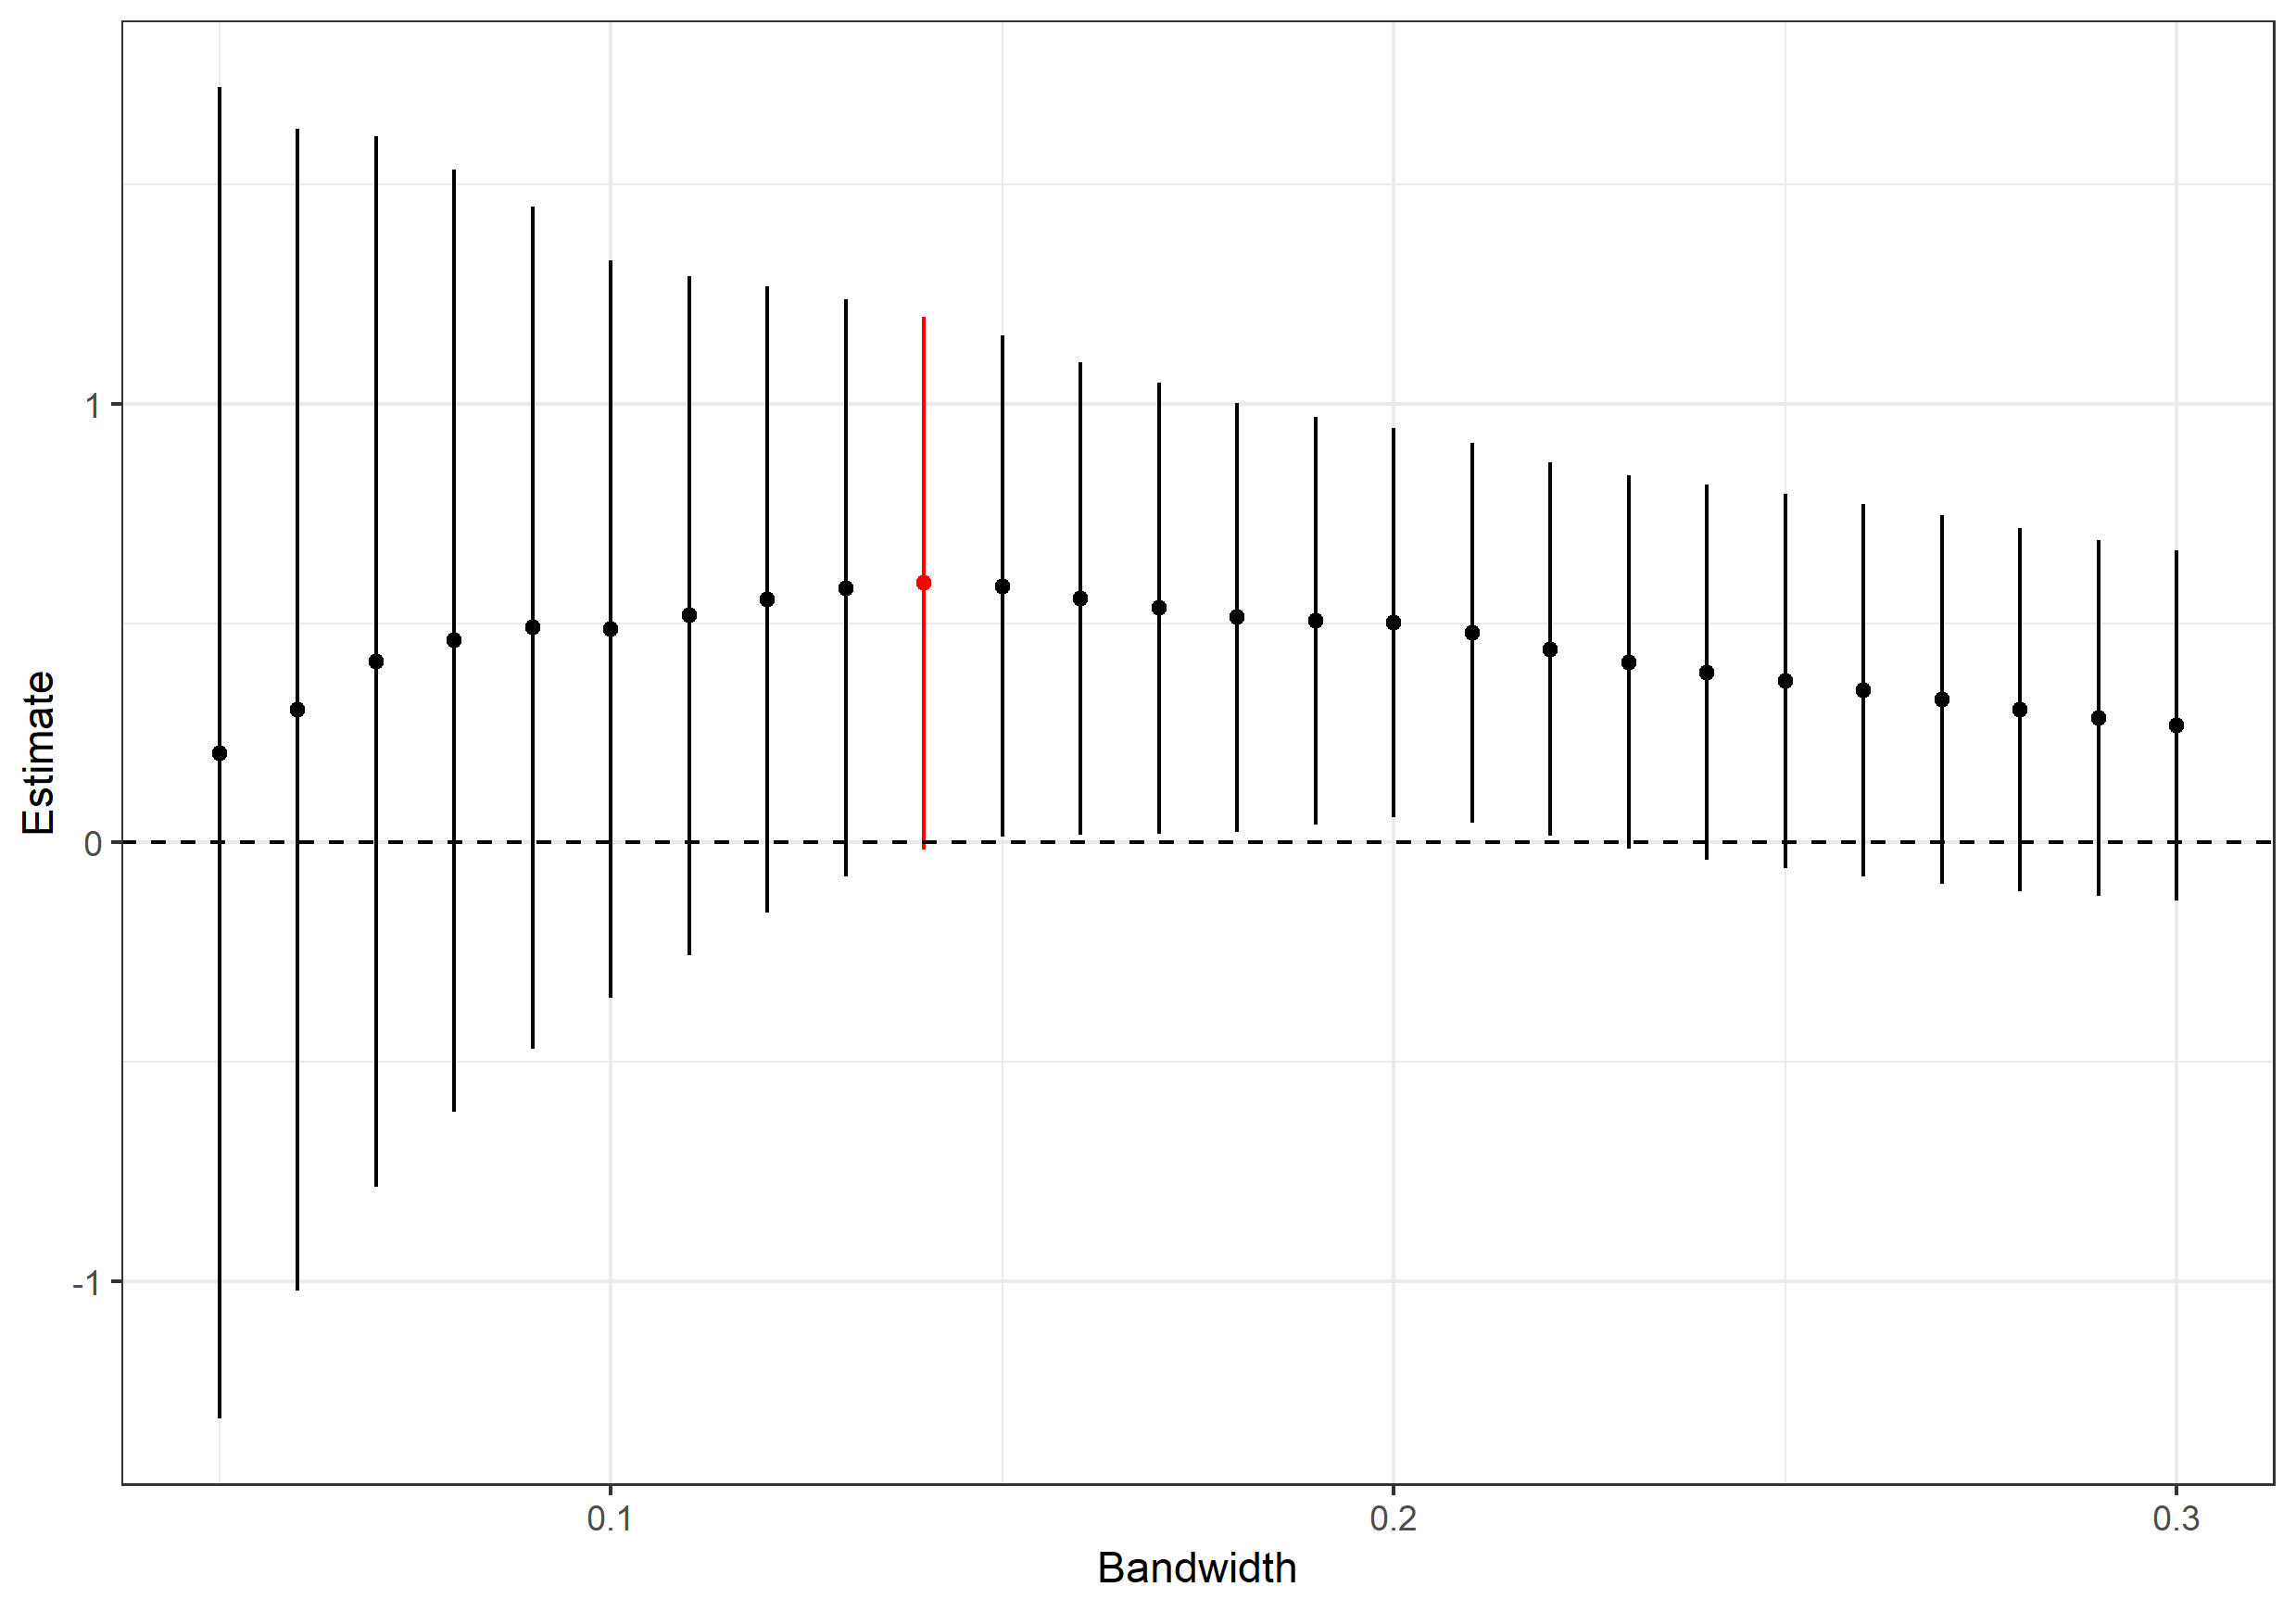
\includegraphics[width=\linewidth]{Figures/bandwidthSensitivity}
	\caption{Sensitivity to choice of bandwidth. Bias-corrected estimates and 95\% confidence intervals (robust standard errors). The CCT optimal bandwidth is plotted in red.}
	\label{fig:bandwidthSensitivity}
	\end{figure}

	\subsection{Sensitivity to Polynomial Order and Kernel Function}

	The \texttt{rdrobust} package defaults to modeling the conditional expectation function with a local-linear and triangular kernel weights. The core result is robust to varying these assumptions, though the 95\% confidence interval is wider (and includes zero) when estimated using a second-order polynomial.
	 
	% Table created by stargazer v.5.2.2 by Marek Hlavac, Harvard University. E-mail: hlavac at fas.harvard.edu
	% Date and time: Fri, Nov 16, 2018 - 2:02:49 PM
	\begin{table}[h] \centering 
		\caption{Regression discontinuity estimates, varying polynomial order and kernel function. Dependent variable = 1-month bond yield regression discontinuity estimates (bias-corrected) with 95\% confidence intervals (robust standard errors) in brackets.} 
		\label{table:RDQuadratic} 
		\begin{tabular}{@{\extracolsep{5pt}}lccc} 
			\\[-1.8ex]\hline 
			\hline \\[-1.8ex] 
			& \multicolumn{3}{c}{\textit{Fragmentation:}} \\ 
			\cline{2-4} 
			\\[-1.8ex] & All & Low & High \\ 
			\\[-1.8ex] & (1) & (2) & (3)\\ 
			\hline \\[-1.8ex] 	
			Linear, Triangular Kernel & 0.145 & 0.592 & $-0.048$ \\ 
			& [-0.12, 0.43] & [-0.01, 1.19] & [-0.32, 0.23] \\ 
			Linear, Uniform Kernel & 0.152 & 0.511 & $-0.077$ \\ 
			& [-0.20, 0.39] & [0.10, 0.92] & [-0.39, 0.23] \\ 
			Quadratic, Triangular Kernel & 0.099 & 0.646 & $-0.109$ \\ 
			& [-0.20, 0.39] & [$-0.11$, 1.40] & [-0.43, 0.21] \\ 
			Quadratic, Uniform Kernel & 0.106 & 0.598 & 0.016 \\ 
			& [-0.19, 0.41] & [$-0.14$, 1.33] & [-0.31, 0.34] \\ 
			\hline \\[-1.8ex] 
			Observations & 316 & 179 & 137 \\ 
			%Bandwidth Estimate $(h)$ & 0.203 & 0.241 & 0.152 \\ 
			\hline 
			\hline \\[-1.8ex] 
		\end{tabular} 
	\end{table}  
	
	\subsection{Dynamic RD Estimates} %TODO Does this make sense, given our theoretical motivation?

        In addition to estimating the short-run effects on bond yields, we can compute a dynamic RD estimate -- actually a series of static estimates -- by varying the time window with which the dependent variable is measured \citep{Cellini2010}. Using this method, we can observe whether a left party plurality yields longer-term changes to bond yields. Furthermore, as a placebo test, we can also examine whether there is an estimated effect on bond yields \textit{prior} to the election. Figure \ref{fig:dynamicRD} illustrates the results from this moving-window RD analysis; the narrow plurality win of a left party appears to have an effect on bond yields that persist for at least a year, peaking at around 10 months, when party fragmentation is low, and, again, no perceptible effect at any time-window in high-fragmentation contexts. 

    \begin{figure} [h]
    	\centering
    	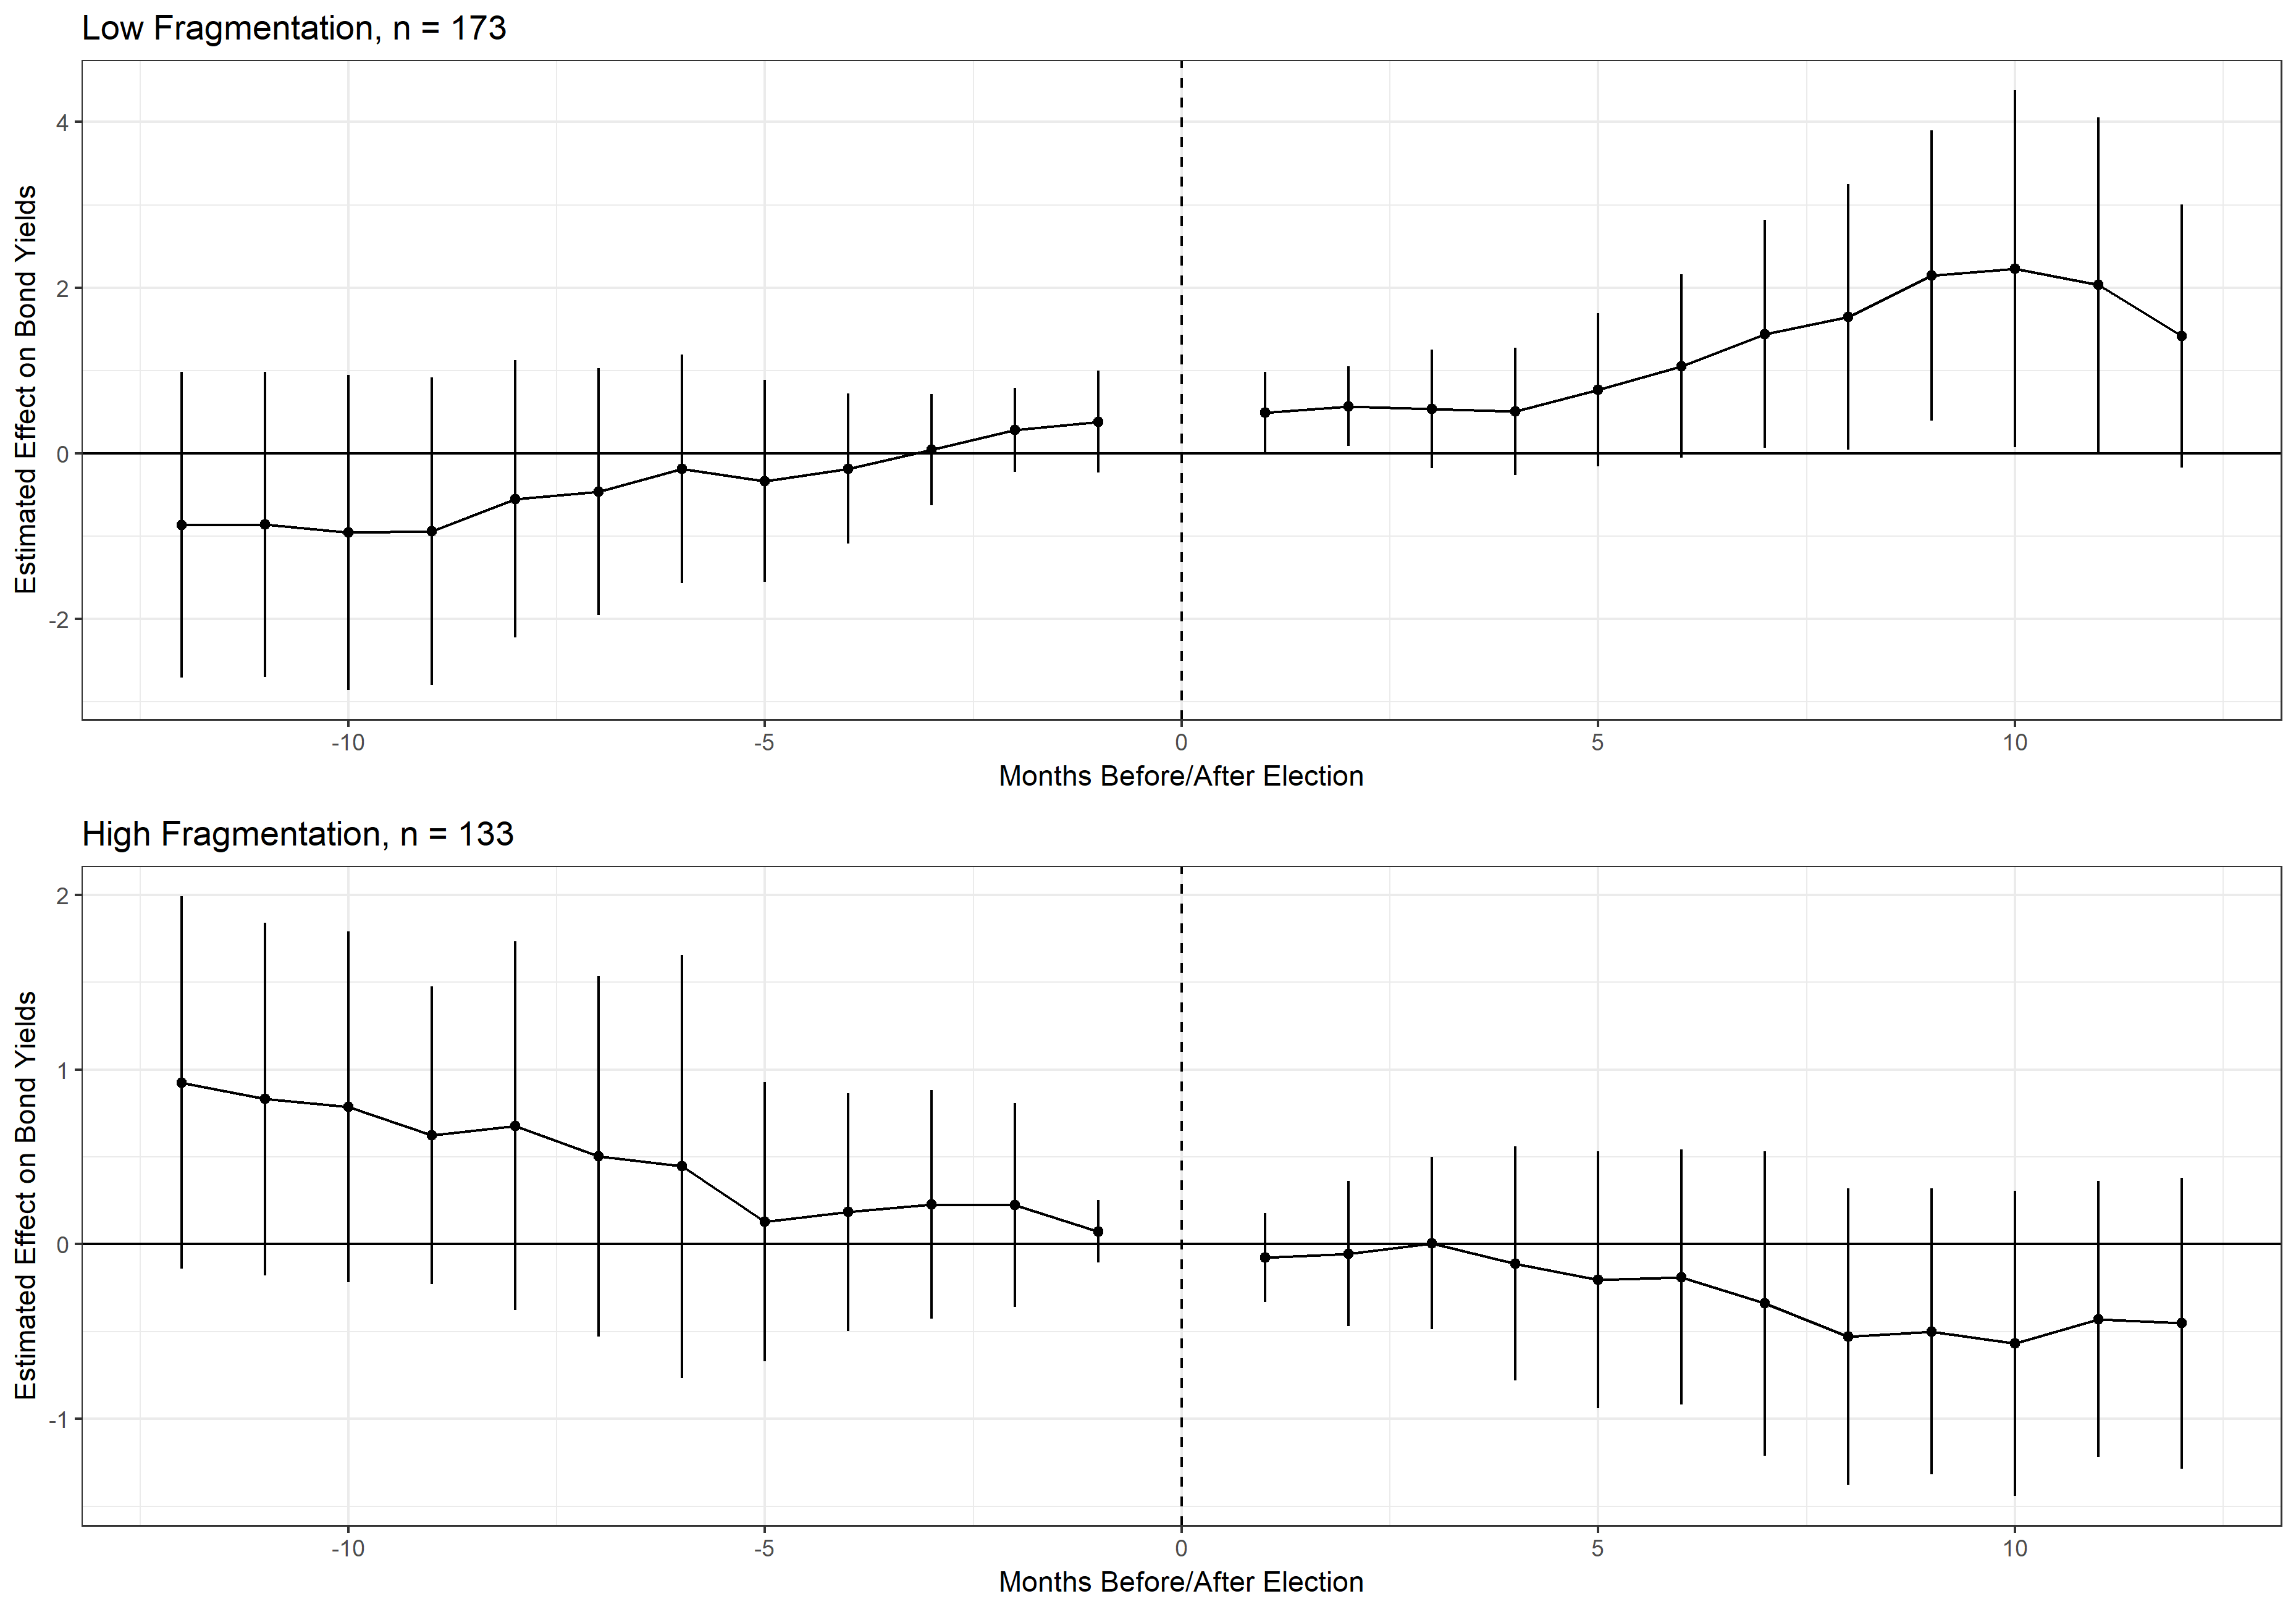
\includegraphics[width=\linewidth]{Figures/dynamicRD}
    	\caption{Dynamic RD estimates. Top panel is low fragmentation elections ($ENPP < 3.5$), bottom     panel is high fragmentation elections ($ENPP > 3.5$).}
    	\label{fig:dynamicRD}
    \end{figure}

\end{appendices}





\end{document}